% Options for packages loaded elsewhere
\PassOptionsToPackage{unicode}{hyperref}
\PassOptionsToPackage{hyphens}{url}
\PassOptionsToPackage{dvipsnames,svgnames,x11names}{xcolor}
%
\documentclass[
  a4paper,
  DIV=11,
  numbers=noendperiod]{scrreprt}

\usepackage{amsmath,amssymb}
\usepackage{iftex}
\ifPDFTeX
  \usepackage[T1]{fontenc}
  \usepackage[utf8]{inputenc}
  \usepackage{textcomp} % provide euro and other symbols
\else % if luatex or xetex
  \usepackage{unicode-math}
  \defaultfontfeatures{Scale=MatchLowercase}
  \defaultfontfeatures[\rmfamily]{Ligatures=TeX,Scale=1}
\fi
\usepackage{lmodern}
\ifPDFTeX\else  
    % xetex/luatex font selection
\fi
% Use upquote if available, for straight quotes in verbatim environments
\IfFileExists{upquote.sty}{\usepackage{upquote}}{}
\IfFileExists{microtype.sty}{% use microtype if available
  \usepackage[]{microtype}
  \UseMicrotypeSet[protrusion]{basicmath} % disable protrusion for tt fonts
}{}
\makeatletter
\@ifundefined{KOMAClassName}{% if non-KOMA class
  \IfFileExists{parskip.sty}{%
    \usepackage{parskip}
  }{% else
    \setlength{\parindent}{0pt}
    \setlength{\parskip}{6pt plus 2pt minus 1pt}}
}{% if KOMA class
  \KOMAoptions{parskip=half}}
\makeatother
\usepackage{xcolor}
\usepackage[top=20mm,bottom=20mm,left=20mm,right=20mm]{geometry}
\setlength{\emergencystretch}{3em} % prevent overfull lines
\setcounter{secnumdepth}{3}
% Make \paragraph and \subparagraph free-standing
\makeatletter
\ifx\paragraph\undefined\else
  \let\oldparagraph\paragraph
  \renewcommand{\paragraph}{
    \@ifstar
      \xxxParagraphStar
      \xxxParagraphNoStar
  }
  \newcommand{\xxxParagraphStar}[1]{\oldparagraph*{#1}\mbox{}}
  \newcommand{\xxxParagraphNoStar}[1]{\oldparagraph{#1}\mbox{}}
\fi
\ifx\subparagraph\undefined\else
  \let\oldsubparagraph\subparagraph
  \renewcommand{\subparagraph}{
    \@ifstar
      \xxxSubParagraphStar
      \xxxSubParagraphNoStar
  }
  \newcommand{\xxxSubParagraphStar}[1]{\oldsubparagraph*{#1}\mbox{}}
  \newcommand{\xxxSubParagraphNoStar}[1]{\oldsubparagraph{#1}\mbox{}}
\fi
\makeatother


\providecommand{\tightlist}{%
  \setlength{\itemsep}{0pt}\setlength{\parskip}{0pt}}\usepackage{longtable,booktabs,array}
\usepackage{calc} % for calculating minipage widths
% Correct order of tables after \paragraph or \subparagraph
\usepackage{etoolbox}
\makeatletter
\patchcmd\longtable{\par}{\if@noskipsec\mbox{}\fi\par}{}{}
\makeatother
% Allow footnotes in longtable head/foot
\IfFileExists{footnotehyper.sty}{\usepackage{footnotehyper}}{\usepackage{footnote}}
\makesavenoteenv{longtable}
\usepackage{graphicx}
\makeatletter
\newsavebox\pandoc@box
\newcommand*\pandocbounded[1]{% scales image to fit in text height/width
  \sbox\pandoc@box{#1}%
  \Gscale@div\@tempa{\textheight}{\dimexpr\ht\pandoc@box+\dp\pandoc@box\relax}%
  \Gscale@div\@tempb{\linewidth}{\wd\pandoc@box}%
  \ifdim\@tempb\p@<\@tempa\p@\let\@tempa\@tempb\fi% select the smaller of both
  \ifdim\@tempa\p@<\p@\scalebox{\@tempa}{\usebox\pandoc@box}%
  \else\usebox{\pandoc@box}%
  \fi%
}
% Set default figure placement to htbp
\def\fps@figure{htbp}
\makeatother
% definitions for citeproc citations
\NewDocumentCommand\citeproctext{}{}
\NewDocumentCommand\citeproc{mm}{%
  \begingroup\def\citeproctext{#2}\cite{#1}\endgroup}
\makeatletter
 % allow citations to break across lines
 \let\@cite@ofmt\@firstofone
 % avoid brackets around text for \cite:
 \def\@biblabel#1{}
 \def\@cite#1#2{{#1\if@tempswa , #2\fi}}
\makeatother
\newlength{\cslhangindent}
\setlength{\cslhangindent}{1.5em}
\newlength{\csllabelwidth}
\setlength{\csllabelwidth}{3em}
\newenvironment{CSLReferences}[2] % #1 hanging-indent, #2 entry-spacing
 {\begin{list}{}{%
  \setlength{\itemindent}{0pt}
  \setlength{\leftmargin}{0pt}
  \setlength{\parsep}{0pt}
  % turn on hanging indent if param 1 is 1
  \ifodd #1
   \setlength{\leftmargin}{\cslhangindent}
   \setlength{\itemindent}{-1\cslhangindent}
  \fi
  % set entry spacing
  \setlength{\itemsep}{#2\baselineskip}}}
 {\end{list}}
\usepackage{calc}
\newcommand{\CSLBlock}[1]{\hfill\break\parbox[t]{\linewidth}{\strut\ignorespaces#1\strut}}
\newcommand{\CSLLeftMargin}[1]{\parbox[t]{\csllabelwidth}{\strut#1\strut}}
\newcommand{\CSLRightInline}[1]{\parbox[t]{\linewidth - \csllabelwidth}{\strut#1\strut}}
\newcommand{\CSLIndent}[1]{\hspace{\cslhangindent}#1}

\KOMAoption{captions}{tableheading}
\makeatletter
\@ifpackageloaded{tcolorbox}{}{\usepackage[skins,breakable]{tcolorbox}}
\@ifpackageloaded{fontawesome5}{}{\usepackage{fontawesome5}}
\definecolor{quarto-callout-color}{HTML}{909090}
\definecolor{quarto-callout-note-color}{HTML}{0758E5}
\definecolor{quarto-callout-important-color}{HTML}{CC1914}
\definecolor{quarto-callout-warning-color}{HTML}{EB9113}
\definecolor{quarto-callout-tip-color}{HTML}{00A047}
\definecolor{quarto-callout-caution-color}{HTML}{FC5300}
\definecolor{quarto-callout-color-frame}{HTML}{acacac}
\definecolor{quarto-callout-note-color-frame}{HTML}{4582ec}
\definecolor{quarto-callout-important-color-frame}{HTML}{d9534f}
\definecolor{quarto-callout-warning-color-frame}{HTML}{f0ad4e}
\definecolor{quarto-callout-tip-color-frame}{HTML}{02b875}
\definecolor{quarto-callout-caution-color-frame}{HTML}{fd7e14}
\makeatother
\makeatletter
\@ifpackageloaded{caption}{}{\usepackage{caption}}
\AtBeginDocument{%
\ifdefined\contentsname
  \renewcommand*\contentsname{Table of contents}
\else
  \newcommand\contentsname{Table of contents}
\fi
\ifdefined\listfigurename
  \renewcommand*\listfigurename{List of Figures}
\else
  \newcommand\listfigurename{List of Figures}
\fi
\ifdefined\listtablename
  \renewcommand*\listtablename{List of Tables}
\else
  \newcommand\listtablename{List of Tables}
\fi
\ifdefined\figurename
  \renewcommand*\figurename{Figure}
\else
  \newcommand\figurename{Figure}
\fi
\ifdefined\tablename
  \renewcommand*\tablename{Table}
\else
  \newcommand\tablename{Table}
\fi
}
\@ifpackageloaded{float}{}{\usepackage{float}}
\floatstyle{ruled}
\@ifundefined{c@chapter}{\newfloat{codelisting}{h}{lop}}{\newfloat{codelisting}{h}{lop}[chapter]}
\floatname{codelisting}{Listing}
\newcommand*\listoflistings{\listof{codelisting}{List of Listings}}
\makeatother
\makeatletter
\makeatother
\makeatletter
\@ifpackageloaded{caption}{}{\usepackage{caption}}
\@ifpackageloaded{subcaption}{}{\usepackage{subcaption}}
\makeatother

\usepackage{bookmark}

\IfFileExists{xurl.sty}{\usepackage{xurl}}{} % add URL line breaks if available
\urlstyle{same} % disable monospaced font for URLs
\hypersetup{
  pdftitle={Design of the Symmetrical OTA},
  pdfauthor={Christian Enz},
  colorlinks=true,
  linkcolor={blue},
  filecolor={Maroon},
  citecolor={Blue},
  urlcolor={Blue},
  pdfcreator={LaTeX via pandoc}}


\title{Design of the Symmetrical OTA}
\usepackage{etoolbox}
\makeatletter
\providecommand{\subtitle}[1]{% add subtitle to \maketitle
  \apptocmd{\@title}{\par {\large #1 \par}}{}{}
}
\makeatother
\subtitle{Version 2}
\author{Christian Enz}
\date{2025-06-05}

\begin{document}
\maketitle

\renewcommand*\contentsname{Table of contents}
{
\hypersetup{linkcolor=}
\setcounter{tocdepth}{2}
\tableofcontents
}

\chapter{Introduction}\label{introduction}

\begin{figure}

\centering{

\pandocbounded{\includegraphics[keepaspectratio]{Figures/Symmetrical_OTA_schematic.png}}

}

\caption{\label{fig-symmetrical_ota_schematic}Schematic of the
symmetrical differential OTA.}

\end{figure}%

\begin{tcolorbox}[enhanced jigsaw, bottomrule=.15mm, colback=white, leftrule=.75mm, toprule=.15mm, opacitybacktitle=0.6, colbacktitle=quarto-callout-note-color!10!white, left=2mm, colframe=quarto-callout-note-color-frame, coltitle=black, bottomtitle=1mm, arc=.35mm, toptitle=1mm, titlerule=0mm, title=\textcolor{quarto-callout-note-color}{\faInfo}\hspace{0.5em}{Note}, breakable, opacityback=0, rightrule=.15mm]

Note that all nMOS transistors in
Figure~\ref{fig-symmetrical_ota_schematic} have an odd number and all
the pMOS transistors an even number which explains the numbering process
(this is the reason why there is no M\textsubscript{6} transistor!).

\end{tcolorbox}

This notebook presents the analysis, design and simulation of the
symmetrical cascode OTA which schematic is presented in
Figure~\ref{fig-symmetrical_ota_schematic}
\citeproc{ref-bib:krummenacher:el:1:4:1981}{{[}1{]}}. The design phase
is using the sEKV model and the inversion coefficient approach
\citeproc{ref-bib:enz:book:2006}{{[}2{]}},
\citeproc{ref-bib:enz:sscmag:autumn:2017}{{[}3{]}},
\citeproc{ref-bib:enz:sscmag:winter:2017}{{[}4{]}}. The symmetrical OTA
is a single-stage OTA having the dominant pole set by the load
capacitance. It therefore doesn't require any compensation capacitance
but can still achieve the gain of a two-stage OTA thanks to the cascode
stages at the output at much lower current consumption. We will see
below that in differential mode the effects of the source
transconductances on the common source node voltage are actually
canceled. In order to minimize the \(V_{GS}\) voltage of
M\textsubscript{1a}-M\textsubscript{1b}, we have chosen to put
M\textsubscript{1a}-M\textsubscript{1b} in a separate well at the cost
of a larger area.

We will start with a detailed analysis of the OTA which will allow to
derive all the design equations that will be used in the design phase.
The OTA is then designed for a given set of specifications for the
chosen IHP SG13G2 130nm BiCMOS technology
\citeproc{ref-bib:ihp:2025}{{[}5{]}}. We have selected this technology
because IHP provides an open source PDK which is then used for the
validation of the design by simulation with ngspice
\citeproc{ref-bib:ngspice:2024}{{[}6{]}} using the PSP compact model
\citeproc{ref-bib:psp103.6:2017}{{[}7{]}} provided by the open source
PDK \citeproc{ref-bib:ihp:2025}{{[}5{]}}.

We now start with the small-signal analysis.

\chapter{Analysis}\label{analysis}

\section{Small-signal analysis}\label{small-signal-analysis}

\begin{figure}

\centering{

\pandocbounded{
\includegraphics[keepaspectratio]{Figures/Small-signal_schematics.png}}

}

\caption{\label{fig-ssc}Small-signal schematic of the symmetrical
cascode OTA.}

\end{figure}%

The small-signal schematic of the symmetrical OTA of
Figure~\ref{fig-symmetrical_ota_schematic} is shown in
Figure~\ref{fig-ssc}. The design of the symmetrical cascode OTA is
similar to the design of the simple OTA, except that there are now more
parasitic poles appearing at the various current mirror nodes. The
small-signal output voltage in open-loop is given by \begin{align}
  \Delta V_{out} =& \frac{A_{dc}}{1+s\,\tau_0} \cdot \left[\frac{\Delta V_{in+}}{1+s\,\tau_{p4}} - \frac{\Delta V_{in-}}{(1+s\,\tau_{p2})(1+s\,\tau_{p3})}\right.\\
  &\left.-\frac{\Delta V_{in+}+\Delta V_{in-}}{2(1+s\,\tau_{p1})} \cdot \left(\frac{1}{1+s\,\tau_{p4}} - \frac{1}{(1+s\,\tau_{p2})(1+s\,\tau_{p3}}\right)\right]
\end{align} where \begin{align}
  A_{dc} &= \frac{G_m}{G_o},\\
  G_m &= A_3 \cdot G_{m1},\\
  G_o &= \frac{G_{ds3b}\,G_{ds7}}{G_{ms7}} + \frac{G_{ds2d}\,G_{ds4}}{G_{ms4}},\\
  \tau_0 &= \frac{C_{out}}{G_o},\\
  C_{out} &= C_L + C_o,\\
  \tau_{p1} &= \frac{C_1}{2 G_{m1}},\\
  \tau_{p2} &= \frac{C_2}{G_{m2}},\\
  \tau_{p3} &= \frac{C_3}{G_{m3}},\\
  \tau_{p4} &= \frac{C_4}{G_{m2}}.
\end{align} \(C_1\), \(C_2\) and \(C_3\) are the total parasitic
capacitances at the current mirrors nodes 1, 2 and 3.

The unity-gain frequency or gain-bandwidth product is defined as
\(\omega_u = 1/\tau_u \triangleq A_{dc}/\tau_0 = G_m/C_{out}\). In most
practical cases, we usually have
\(\tau_0 \gg \tau_{p2}, \tau_{p3}, \tau_{p4} > \tau_{p1}\).

For a differential input voltage
\(\Delta V_{id}=\Delta V_{in+}-\Delta V_{in-}\) with a constant
common-mode voltage \(V_{ic}\) and hence
\(\Delta V_{ic} = (\Delta V_{in+} + \Delta V_{in-})/2=0\),
\(\Delta V_{in+} = -\Delta V_{in-} = \Delta V_{id}/2\), the differential
mode small-signal open-loop gain reduces to \begin{equation}
  A_{dm}(s) \triangleq \frac{\Delta V_{out}}{\Delta V_{id}} = \frac{1}{2} \cdot \frac{A_{dc}}{1+s\,\tau_0} \cdot \left[\frac{1}{1+s\,\tau_{p4}} - \frac{1}{(1+s\,\tau_{p2})(1+s\,\tau_{p3})}\right].
\end{equation}

The small-signal output voltage \(\Delta V_{out}\) can also be written
as \begin{equation}\label{eqn:DVout_F_G}
  \Delta V_{out} = \frac{A_{dc}}{1+s\,\tau_0} \cdot \left[F(s) \cdot \Delta V_{in+} - G(s) \cdot \Delta V_{in-}\right],
\end{equation} where \begin{align}
  F(s) &= \frac{1}{1+s\,\tau_{p4}} - \frac{1}{2}\,\frac{1}{1+s\,\tau_{p1}} \cdot \left[\frac{1}{1+s\,\tau_{p4}} - \frac{1}{(1+s\,\tau_{p2})(1+s\,\tau_{p3})}\right],\\
  G(s) &= \frac{1}{(1+s\,\tau_{p2})(1+s\,\tau_{p3})} + \frac{1}{2}\,\frac{1}{1+s\,\tau_{p1}} \cdot \left[\frac{1}{1+s\,\tau_{p4}} - \frac{1}{(1+s\,\tau_{p2})(1+s\,\tau_{p3})}\right].
\end{align}

From \eqref{eqn:DVout_F_G} we see that the time constant \(\tau_0\)
introduces a \(-90^\circ\) phase shift. Hence if the desired phase
margin is at least \(60^\circ\), the additional phase shift introduced
by the smaller time constants \(\tau_{p1}\), \(\tau_{p2}\),
\(\tau_{p3}\) and \(\tau_{p4}\) should not exceed \(30^\circ\). In this
range, the product
\((1+s\,\tau_{p1})(1+s\,\tau_{p2})(1+s\,\tau_{p3})(1+s\,\tau_{p4})\) can
be expanded and approximated by neglecting all the order terms higher
than the first order term in \(s\) \begin{equation}
  \prod_{k=1}^{4} (1+s\,\tau_{pk}) \cong 1 + s \, \sum_{k=1}^{4} \tau_{pk}.
\end{equation} The above approximation gives a good estimation of the
phase shift \(\phi\) for \(\phi < 30^\circ\), which correspond to the
following frequency range \begin{equation}
  \omega \leq \left(2\sum_{k=1}^{4} \tau_{pk}\right)^{-1}.
\end{equation} Using the above approximation leads to \begin{equation}
  F(s) \cong G(s) \cong \frac{1+s\,\tau_n}{1 + s\,\tau_d},
\end{equation} where \begin{align}
  \tau_n &= \tau_{p1} + \frac{\tau_{p2}+\tau_{p3}+\tau_{p4}}{2},\\
  \tau_d &= \tau_{p1}+\tau_{p2}+\tau_{p3}+\tau_{p4}.
\end{align}

For \(\omega \leq 1/(2 \tau_d)\), the above expression can be further
simplified considering that \begin{equation}
  \frac{1+s\,\tau_n}{1 + s\,\tau_d} \cong \frac{1}{1 + s\,(\tau_d-\tau_n)}
\end{equation} where \begin{equation}
  \tau_d-\tau_n = \frac{\tau_{p2}+\tau_{p3}+\tau_{p4}}{2} = \frac{\tau_p}{2}.
\end{equation}

\(F(s)\) and \(G(s)\) become \begin{equation}
  F(s) \cong G(s) \cong \frac{1}{1+s\,\frac{\tau_p}{2}},
\end{equation} which is valid for
\(\omega \leq 1/(2 \tau_d) =1/(2(\tau_{p2}+\tau_p))\).

The simplified differential transfer function is then given by
\begin{equation}
  A_{dm}(s) \cong \frac{A_{dc}}{\left(1+s\,\tau_0\right)\left(1+s\,\frac{\tau_p}{2}\right)} = \frac{A_{dc}}{\left(1+\frac{s}{\omega_0}\right)\left(1+\frac{s}{\omega_p}\right)}
\end{equation} with \(\omega_0 \triangleq 1/\tau_0\) and
\(\omega_p \triangleq 2/\tau_p\) where it is assumed that
\(\tau_p = \tau_{p2}+\tau_{p3}+\tau_{p4} \ll \tau_0\).
\(\omega_0 \triangleq 1/\tau_0 \ll \omega_p\) is the dominant pole which
is set by the load capacitance at the OTA output, whereas
\(\omega_p \triangleq 2/\tau_p\) represents the non-dominant pole
related to all the time constants due to the parasitic capacitances at
the current mirror nodes.

The transfer function can be further simplified as \begin{equation}
  A_{dm}(s) \cong \frac{1}{s\,\tau_u\left(1+s\,\frac{\tau_p}{2}\right)} = \frac{1}{\frac{s}{\omega_u}\left(1+\frac{s}{\omega_p}\right)}
\end{equation}

where \(\omega_u = 1/\tau_u = A_{dc} \cdot \omega_0 = G_m/C_{out}\) is
the unity gain frequency or the gain-bandwidth product \(GBW\) which is
set by the OTA transconductance \(G_m\) and the load capacitance
\(C_{out}\).

\section{Noise analysis}\label{noise-analysis}

We have seen that the noise of the cascode transistors
M\textsubscript{4} and M\textsubscript{7} can actually be neglected.
Remembering that \(A_3=A_1 \cdot A_2\), the PSD of the output noise
current is given by \begin{equation}
  S_{I_{nout}} = A_3^2\,\left(S_{I_{n1a}}+S_{I_{n1b}}+S_{I_{n2a}}+S_{I_{n2b}}\right) + A_2^2\,\left(S_{I_{n2c}}+S_{I_{n3a}}\right)+S_{I_{n2d}}+S_{I_{n3b}}
\end{equation} or if we express the output PSD in terms of the output
noise conductance \begin{equation}
  S_{I_{nout}} =4 kT \cdot G_{nout}
\end{equation} where \begin{equation}
  G_{nout} = 2 A_3^2 \cdot (G_{n1}+G_{n2}) + A_2^2 \cdot (G_{n2c}+G_{n3a}) + G_{n2d} + G_{n3b}
\end{equation} where we have assumed that M\textsubscript{1a} and
M\textsubscript{1b} and M\textsubscript{2a} and M\textsubscript{2b} are
identical. The \(G_{ni}\) are given by \begin{equation}
  G_{ni} = \gamma_{ni} \cdot G_{mi} + G_{mi}^2 \cdot \frac{\rho_i}{W_i\,L_i\,f} \qquad \textsf{for all transistors}.
\end{equation}

The input-referred noise resistance \(R_{nin}\) is then given by
\begin{equation}
  R_{nin} \triangleq \frac{G_{nout}}{A_3^2 \cdot G_{m1}^2} = \frac{2(G_{n1}+G_{n2})}{G_{m1}^2} + \frac{G_{n2c}+G_{n3a}}{A_1^2 \cdot G_{m1}^2} + \frac{G_{n2d}+G_{n3b}}{A_3^2 \cdot G_{m1}^2}
\end{equation} where we have used \(A_3=A_1 \cdot A_2\). As expected, we
see that the noise contribution to the input-referred noise of
M\textsubscript{2d} and M\textsubscript{3b} is divided by \(A_3^2\) and
that from M\textsubscript{2c} and M\textsubscript{3a} is divided by
\(A_1^2\).

We now look at the input-referred thermal and flicker noise separately.

\subsection{Input-referred thermal
noise}\label{input-referred-thermal-noise}

The input-referred thermal noise resistance is given by \begin{equation}
  R_{nth} = \frac{2 \gamma_{n1}}{G_{m1}} \cdot (1 + \eta_{th})
\end{equation} where \begin{align}
  \eta_{th} &= \frac{\gamma_{n2}}{\gamma_{n1}}\,\frac{G_{m2}}{G_{m1}} + \frac{1}{2 A_1^2}\,\left(\frac{\gamma_{n2c}}{\gamma_{n1}}\,\frac{G_{m2c}}{G_{m1}} + \frac{\gamma_{n3a}}{\gamma_{n1}}\,\frac{G_{m3a}}{G_{m1}}\right)\\
  &+\frac{1}{2 A_3^2}\,\left(\frac{\gamma_{n2d}}{\gamma_{n1}}\,\frac{G_{m2d}}{G_{m1}} +\frac{\gamma_{n3b}}{\gamma_{n1}}\,\frac{G_{m3b}}{G_{m1}}\right)
\end{align} represents the contributions to the input-referred thermal
noise of the current mirrors relative to that of the differential pair.
Now \(G_{m2c}=A_1 \cdot G_{m2a}=A_1 \cdot G_{m2}\),
\(G_{m3b}=A_2 \cdot G_{m3a}=A_2 \cdot G_{m3}\) and
\(G_{m2d}=A_3 \cdot G_{m2b} = A_3 \cdot G_{m2}\), and assuming that
\(\gamma_{n2a}=\gamma_{n2b}\cong\gamma_{n2c}\cong\gamma_{n2d}=\gamma_{n2}\)
and \(\gamma_{n3a}\cong\gamma_{n3b}=\gamma_{n3}\), then \(\eta_{th}\)
reduces to \begin{equation}
  \eta_{th} = \frac{\gamma_{n2}}{2\gamma_{n1}}\,\frac{G_{m2}}{G_{m1}} \left(2+\frac{1}{A_1}+\frac{1}{A_3}\right) +\frac{1}{2 A_1^2}\,\frac{\gamma_{n3}}{\gamma_{n1}}\,\frac{G_{m3}}{G_{m1}} \left(1+\frac{1}{A_2}\right)
\end{equation}

In the case of unity current gains \(A_1=A_2=A_3=1\), \(\eta_{th}\)
simplifies further to \begin{equation}
  \eta_{th} = 2 \frac{\gamma_{n2}}{\gamma_{n1}}\,\frac{G_{m2}}{G_{m1}} + \frac{\gamma_{n3}}{\gamma_{n1}}\,\frac{G_{m3}}{G_{m1}}
\end{equation} Of course in the design process, we will try to minimize
\(\eta_{th}\) so that the dominant contribution to the input-referred
thermal noise comes from the differential pair
M\textsubscript{1a}-M\textsubscript{1b}.

We can also introduce the OTA thermal noise excess factor as
\begin{equation}
  \gamma_{ota} \triangleq G_m \cdot R_{nth},
\end{equation} where \(G_m = A_3 \cdot G_{m1}\) is the OTA
transconductance. This results in \begin{equation}
  \gamma_{ota} = 2 A_3 \cdot \gamma_{n1} \cdot (1 + \eta_{th}).
\end{equation} We see that introducing some current gains larger than
one in the current mirrors allows to reduce the contributions of
transistors M\textsubscript{2c}-M\textsubscript{2d} and
M\textsubscript{3a}-M\textsubscript{3b}, but on the other hand increases
the contribution of the differential pair and hence degrading
(i.e.~increasing) the OTA thermal noise excess factor \(\gamma_{ota}\).

For \(G_{m1} \gg G_{m2}\) and \(G_{m1} \gg G_{m3}\), the noise is
dominated by the differential pair and \begin{equation}
  \gamma_{ota} \cong 2 A_3 \cdot \gamma_{n1}.
\end{equation}

For unity current gains \(A_1=A_2=A_3=1\), the OTA thermal noise excess
factor \(\gamma_{ota}\) reduces to \begin{equation}
  \gamma_{ota} \cong 2 \gamma_{n1}.
\end{equation}

\subsection{Input-referred flicker
noise}\label{input-referred-flicker-noise}

The input-referred flicker noise resistance is given by \begin{align}
  f \cdot R_{nfl} =& \frac{2 \rho_n}{W_1 L_1} + \rho_p\,\left(\frac{G_{m2}}{G_{m1}}\right)^2 \left(\frac{2}{W_2 L_2}+\frac{1}{W_{2c} L_{2c}}+\frac{1}{W_{2d} L_{2d}}\right)\\
  &+ \frac{\rho_n}{A_1^2}\left(\frac{G_{m3}}{G_{m1}}\right)^2\left(\frac{1}{W_{3a} L_{3a}}+\frac{1}{W_{3b} L_{3b}}\right)
\end{align} which can be written as \begin{equation}
  R_{nfl} = \frac{2 \rho_n}{W_1 L_1 f} \cdot (1 + \eta_{fl})
\end{equation} where \(\eta_{fl}\) represents the contributions to the
input-referred flicker noise resistance of the current mirrors relative
to that of the differential pair \begin{align}
  \eta_{fl} =& \frac{\rho_p}{2\rho_n}\,\left(\frac{G_{m2}}{G_{m1}}\right)^2 \left(\frac{2 W_1 L_1}{W_2 L_2}+\frac{W_1 L_1}{W_{2c} L_{2c}}+\frac{W_1 L_1}{W_{2d} L_{2d}}\right)\\
  &+ \frac{1}{2 A_1^2}\left(\frac{G_{m3}}{G_{m1}}\right)^2\left(\frac{W_1 L_1}{W_{3a} L_{3a}}+\frac{W_1 L_1}{W_{3b} L_{3b}}\right).
\end{align}

For \(A_1=A_2=A_3=1\), \(W_{2a}=W_{2b}=W_{2c}=W_{2d}=W_2\),
\(L_{2a}=L_{2b}=L_{2c}=L_{2d}=L_2\), \(W_{3a}=W_{3b}=W_3\) and
\(L_{3a}=L_{3b}=L_3\) reduces to \begin{equation}
  \eta_{fl} = 2\frac{\rho_p}{\rho_n}\,\left(\frac{G_{m2}}{G_{m1}}\right)^2\,\frac{W_1 L_1}{W_2 L_2} + \left(\frac{G_{m3}}{G_{m1}}\right)^2\,\frac{W_1 L_1}{W_3 L_3}.
\end{equation} Similarly to thermal noise, in the design process we will
try to minimize \(\eta_{fl}\) in order to reduce the input-referred
flicker noise to the contribution of the differential pair
M\textsubscript{1a}-M\textsubscript{1b}.

The corner frequency is obtained by equating \(R_{nfl(f_k)} = R_{nth}\)
resulting in \begin{equation}
  f_k = \frac{\rho_n\,G_{m1}}{W_1\,L_1\,\gamma_{n1}} \cdot \frac{1+\eta_{fl}}{1+\eta_{th}}.
\end{equation}

\section{Input-referred offset
voltage}\label{input-referred-offset-voltage}

The input-referred random offset voltage can be obtained in a similar
way than noise. The variance of the input-referred offset voltage is
given by \begin{equation}\label{eqn:vos}
  \sigma_{V_{os}}^2 = \sigma_{V_{T1}}^2 \cdot (1 + \xi_{V_T}) + \left(\frac{I_b}{G_{m1}}\right)^2 \cdot \sigma_{\beta_1}^2 \cdot (1 + \xi_{\beta})
\end{equation} where \(\xi_{V_T}\) represents the \(V_T\)-mismatch
contributions to the input-referred offset of the current mirrors
relative to that of the differential pair
\begin{equation}\label{eqn:xivt1}
  \xi_{V_T} = 2 \left(\frac{G_{m2}}{G_{m1}}\right)^2 \cdot \frac{\sigma_{V_{T2}}^2}{\sigma_{V_{T1}}^2} + \left(\frac{G_{m3}}{A_1\,G_{m1}}\right)^2 \cdot \frac{\sigma_{V_{T3}}^2}{\sigma_{V_{T1}}^2}
\end{equation} and \(\xi_{\beta}\) represents the \(\beta\)-mismatch
contributions to the input-referred offset of the current mirrors
relative to that of the differential pair
\begin{equation}\label{eqn:xibeta1}
  \xi_{\beta} = 2 \frac{\sigma_{\beta_2}^2}{\sigma_{\beta_1}^2} + \frac{\sigma_{\beta_3}^2}{A_1^2\,\sigma_{\beta_1}^2}
\end{equation} with \begin{align}
  \sigma_{V_{T1}}^2 &= \frac{A_{VTn}^2}{W_1 L_1},\\
  \sigma_{V_{T2}}^2 &= \frac{A_{VTp}^2}{W_2 L_2},\\
  \sigma_{V_{T3}}^2 &= \frac{A_{VTn}^2}{W_3 L_3},
\end{align} and \begin{align}
  \sigma_{\beta_1}^2 &= \frac{A_{\beta n}^2}{W_1 L_1},\\
  \sigma_{\beta_2}^2 &= \frac{A_{\beta p}^2}{W_2 L_2},\\
  \sigma_{\beta_3}^2 &= \frac{A_{\beta n}^2}{W_3 L_3}.
\end{align}

Replacing in \eqref{eqn:xivt1} and \eqref{eqn:xibeta1} results in
\begin{equation}\label{eqn:xivt2}
  \xi_{V_T} = 2 \left(\frac{G_{m2}}{G_{m1}}\right)^2 \cdot \left(\frac{A_{VTp}}{A_{VTn}}\right)^2 \cdot \frac{W_1 L_1}{W_2 L_2} + \left(\frac{G_{m3}}{A_1\,G_{m1}}\right)^2 \cdot \frac{W_1 L_1}{W_3 L_3}
\end{equation} and \begin{equation}\label{eqn:xibeta2}
  \xi_{\beta} = 2 \left(\frac{A_{\beta p}}{A_{\beta n}}\right)^2 \cdot \frac{W_1 L_1}{W_2 L_2} + \frac{1}{A_1^2}\,\frac{W_1 L_1}{W_3 L_3}
\end{equation}

Similarly to the flicker noise, the input-referred offset (variance or
standard deviation) can be reduced by increasing the differential pair
M\textsubscript{1a}-M\textsubscript{1b} area \(W_1 L_1\) but at the same
time also increasing the area of the current mirrors \(W_2 L_2\) (and
hence \(W_{2c} L_{2c}\) and \(W_{2d} L_{2d}\)) and depending on \(A_1\)
also the area of the current mirror
M\textsubscript{3a}-M\textsubscript{3b} \(W_{3a} L_{3a}\) and
\(W_{3b} L_{3b}\). This obviously comes at the cost of increased
parasitic capacitances at nodes 2, 3 and 4 that will unavoidably reduce
the phase margin.

Having done the small-signal, noise and offset analysis, we can now
proceed with the design.

\chapter{Design}\label{design}

\section{Specifications}\label{specifications}

The OTA specifications are given in Table~\ref{tbl-ota_specs}.

\begin{tcolorbox}[enhanced jigsaw, bottomrule=.15mm, colback=white, leftrule=.75mm, toprule=.15mm, opacitybacktitle=0.6, colbacktitle=quarto-callout-warning-color!10!white, left=2mm, colframe=quarto-callout-warning-color-frame, coltitle=black, bottomtitle=1mm, arc=.35mm, toptitle=1mm, titlerule=0mm, title=\textcolor{quarto-callout-warning-color}{\faExclamationTriangle}\hspace{0.5em}{Warning}, breakable, opacityback=0, rightrule=.15mm]

An important limitation of the IHP SC13G2 BiCMOS technology
\citeproc{ref-bib:ihp:2025}{{[}5{]}} is the high output conductance and
hence the limited intrinsic gain of nMOS transistors. Because of this,
the specification on the DC gain, that was initially set to 80 dB, has
been downgraded to 70 dB.

\end{tcolorbox}

\begin{tcolorbox}[enhanced jigsaw, bottomrule=.15mm, colback=white, leftrule=.75mm, toprule=.15mm, opacitybacktitle=0.6, colbacktitle=quarto-callout-note-color!10!white, left=2mm, colframe=quarto-callout-note-color-frame, coltitle=black, bottomtitle=1mm, arc=.35mm, toptitle=1mm, titlerule=0mm, title=\textcolor{quarto-callout-note-color}{\faInfo}\hspace{0.5em}{Note}, breakable, opacityback=0, rightrule=.15mm]

The specifications given in Table~\ref{tbl-ota_specs} are simplified
specifications. They are mainly targeting the achievement of a certain
gain-bandwidth product \(GBW\) and DC gain at lowest current
consumption. The \(GBW\) sets the differential pair transconductance
while the DC gain sets the output conductance. There is an additional
specification on the random input-referred offset voltage which, if not
met, might eventually require to increase the transistors area. There
are no specifications on thermal noise since the transconductance is set
by the \(GBW\). There are no specifications on the flicker noise but if
the corner frequency was set lower this would required to increase the
transistors area. There are also no specifications on the slew-rate,
which might be small because of the low-power objective. Finally, there
are many more specifications such as CMRR, PSRR, input common-mode
voltage range, output-voltage swing, etc\ldots{} that are not discussed
in this example.

\end{tcolorbox}

\begin{longtable}[]{@{}lccc@{}}

\caption{\label{tbl-ota_specs}OTA specifications.}

\tabularnewline

\toprule\noalign{}
Specification & Symbol & Value & Unit \\
\midrule\noalign{}
\endhead
\bottomrule\noalign{}
\endlastfoot
Minimum DC gain & \(A_{{dc}}\) & 70 & \(dB\) \\
Minimum gain-bandwidth product & \(GBW\) & 1 & \(MHz\) \\
Load capacitance & \(C_L\) & 1 & \(pF\) \\
Maximum input-referred random offset voltage & \(V_{{os}}\) & 10 &
\(mV\) \\
Phase margin & \(PM\) & 60 & \(^{\circ}\) \\

\end{longtable}

\section{Process}\label{process}

We will design the cascode gain stage for the open source IHP 13G2
BiCMOS process \citeproc{ref-bib:ihp:2025}{{[}5{]}}. The physical
parameters are given in Table~\ref{tbl-physics_param}, the global
process parameters in Table~\ref{tbl-process_param} and finally the
MOSFET parameters in Table~\ref{tbl-mos_param}.

\begin{tcolorbox}[enhanced jigsaw, bottomrule=.15mm, colback=white, leftrule=.75mm, toprule=.15mm, opacitybacktitle=0.6, colbacktitle=quarto-callout-warning-color!10!white, left=2mm, colframe=quarto-callout-warning-color-frame, coltitle=black, bottomtitle=1mm, arc=.35mm, toptitle=1mm, titlerule=0mm, title=\textcolor{quarto-callout-warning-color}{\faExclamationTriangle}\hspace{0.5em}{Warning}, breakable, opacityback=0, rightrule=.15mm]

The matching parameters for IHP 130nm are unknown. We will use those
from a generic 180nm technology.

\end{tcolorbox}

\begin{longtable}[]{@{}ccc@{}}

\caption{\label{tbl-physics_param}Physical parameters}

\tabularnewline

\toprule\noalign{}
Parameter & Value & Unit \\
\midrule\noalign{}
\endhead
\bottomrule\noalign{}
\endlastfoot
\(T\) & 300 & \(K\) \\
\(U_T\) & 25.865 & \(mV\) \\

\end{longtable}

\begin{longtable}[]{@{}cccl@{}}

\caption{\label{tbl-process_param}Process parameters.}

\tabularnewline

\toprule\noalign{}
Parameter & Value & Unit & Comment \\
\midrule\noalign{}
\endhead
\bottomrule\noalign{}
\endlastfoot
\(t_{{ox}}\) & 2.24 & \(nm\) & SiO\textsubscript{2} oxyde thickness \\
\(C_{{ox}}\) & 15.413 & \(\frac{{fF}}{{\mu m^2}}\) & Oxyde capacitance
per unit area \\
\(V_{{DD}}\) & 1.2 & \(V\) & Nominal supply voltage \\
\(L_{{min}}\) & 130 & \(nm\) & Minimum drawn gate length \\
\(W_{{min}}\) & 150 & \(nm\) & Minimum drawn gate width \\
\(z_1\) & 340 & \(nm\) & Minimum outer diffusion width \\
\(z_2\) & 389 & \(nm\) & Minimum diffusion width between two fingers \\

\end{longtable}

\begin{longtable}[]{@{}rccl@{}}

\caption{\label{tbl-mos_param}Transistors parameters.}

\tabularnewline

\toprule\noalign{}
Parameter & nMOS & pMOS & Unit \\
\midrule\noalign{}
\endhead
\bottomrule\noalign{}
\endlastfoot
Length and width correction parameters for current & & & \\
\(DL\) & 59 & 51 & \(nm\) \\
\(DW\) & -20 & 30 & \(nm\) \\
Length and width correction for intrinsic and overlap capacitances & &
& \\
\(DLCV\) & 93 & 146 & \(nm\) \\
\(DWCV\) & -10 & 15 & \(nm\) \\
Length and width correction parameter for fringing capacitances & & & \\
\(DLGCV\) & 34 & 96 & \(nm\) \\
\(DWGCV\) & 10 & -15 & \(nm\) \\
Long-channel sEKV parameters parameters & & & \\
\(n\) & 1.22 & 1.23 & - \\
\(I_{{spec\Box}}\) & 708 & 245 & \(nA\) \\
\(V_{{T0}}\) & 246 & 365 & \(mV\) \\
Short-channel sEKV parameters parameters & & & \\
\(L_{{sat}}\) & 7.1 & 24.9 & \(nm\) \\
\(\lambda\) & 1.375 & 6.078 & \(\frac{{V}}{{\mu m}}\) \\
Junction capacitances parameters & & & \\
\(C_J\) & 0.976 & 0.863 & \(\frac{{fF}}{{\mu m^2}}\) \\
\(C_{{JSWSTI}}\) & 0.025 & 0.032 & \(\frac{{fF}}{{\mu m}}\) \\
\(C_{{JSWGAT}}\) & 0.03 & 0.027 & \(\frac{{fF}}{{\mu m}}\) \\
Overlap capacitances parameters & & & \\
\(C_{{GSo}}\) & 0.453 & 0.443 & \(\frac{{fF}}{{\mu m}}\) \\
\(C_{{GDo}}\) & 0.453 & 0.443 & \(\frac{{fF}}{{\mu m}}\) \\
\(C_{{GBo}}\) & 0 & 0.022 & \(\frac{{fF}}{{\mu m}}\) \\
Fringing capacitances parameters & & & \\
\(C_{{GSf}}\) & 0.2 & 0.1 & \(\frac{{fF}}{{\mu m}}\) \\
\(C_{{GDf}}\) & 0.2 & 0.1 & \(\frac{{fF}}{{\mu m}}\) \\
Flicker noise parameters & & & \\
\(K_F\) & 2.208e-24 & 1.2e-23 & \(V A s\) \\
\(AF\) & 1 & 1 & - \\
\(\rho\) & 0.008642 & 0.04697 & \(\frac{{V m^2}}{{A s}}\) \\
Matching parameters & & & \\
\(A_{{VT}}\) & 5 & 5 & \(mV \cdot \mu m\) \\
\(A_{{\beta}}\) & 1 & 1 & \(\% \cdot \mu m\) \\

\end{longtable}

\section{Design procedure}\label{design-procedure}

\begin{tcolorbox}[enhanced jigsaw, bottomrule=.15mm, colback=white, leftrule=.75mm, toprule=.15mm, opacitybacktitle=0.6, colbacktitle=quarto-callout-important-color!10!white, left=2mm, colframe=quarto-callout-important-color-frame, coltitle=black, bottomtitle=1mm, arc=.35mm, toptitle=1mm, titlerule=0mm, title=\textcolor{quarto-callout-important-color}{\faExclamation}\hspace{0.5em}{Important}, breakable, opacityback=0, rightrule=.15mm]

For this process, the transistor dimensions are rounded to 10nm. We also
will ignore the length and width reduction parameters \(DL\) and \(DW\).
The main reason is that most of the transistor length and width are
sufficiently large that ignoring these parameters has little impact.

\end{tcolorbox}

We need to start with choosing the curent gain \(A_3\). We have seen
that having a current gain \(A_3 > 1\) improves the transconductance but
at the cost of a higher thermal noise excess factor \(\gamma_{ota}\). We
therefore will set to \(A_1 =\) 1, \(A_2 =\) 1 and \(A_3 =\) 1. Since
\(A_1 = A_2 = A_3 = 1\), transistors M\textsubscript{2a},
M\textsubscript{2b}, M\textsubscript{2c} and M\textsubscript{2d} are all
identical and so are M\textsubscript{3a} and M\textsubscript{3b}. We
therefore have the following variables:

\begin{itemize}
\tightlist
\item
  M\textsubscript{1a}-M\textsubscript{1b}: \(W_1\), \(L_1\) and \(I_b\).
  Note that the current \(I_b\) is set by \(G_{m1}\) because
  M\textsubscript{1a}-M\textsubscript{1b} are biased in weak inversion,
\item
  M\textsubscript{2a}-M\textsubscript{2c} and
  M\textsubscript{2b}-M\textsubscript{2d}: \(IC_2\), \(W_2\) and \(L_2\)
  since the current is already set,
\item
  M\textsubscript{3a}-M\textsubscript{3b}: \(IC_3\), \(W_3\) and \(L_3\)
  since the current is already set,
\item
  M\textsubscript{4}: \(IC_4\), \(W_4\) and \(L_4\) since the current is
  already set,
\item
  M\textsubscript{7}: \(IC_7\), \(W_7\) and \(L_7\) since the current is
  already set,
\item
  M\textsubscript{5a}-M\textsubscript{5b}: \(IC_5\), \(W_5\) and \(L_5\)
  since the current is already set.
\end{itemize}

We start sizing the differential pair
M\textsubscript{1a}-M\textsubscript{1b}.

\subsection{\texorpdfstring{Sizing the differential pair
M\textsubscript{1a}-M\textsubscript{1b}}{Sizing the differential pair M1a-M1b}}\label{sizing-the-differential-pair-m1a-m1b}

In this example there is no specification on the input-referred white
noise. Therefore the transconductance \(G_{m1}\) is set by the
gain-bandwidth product according to \begin{equation}
  GBW = \frac{G_{m1}}{2 \pi C_{out}},
\end{equation} where \(G_{m1}\) is the gate transconductance of
M\textsubscript{1a} and M\textsubscript{1b} and \(C_{out}\) the total
output capacitance \begin{equation}
  C_{out} = C_L + C_o
\end{equation} with \(C_L\) the specified load capacitance and \(C_o\)
the parasitic capacitance at the output node.

In order to minimize the input-referred noise and offset, the input
differential pair should be biased in weak inversion. The
transconductance \(G_{m1}\) in deep weak inversion is then given by
\begin{equation}
  G_{m1} = \frac{I_b}{n\,U_T}.
\end{equation} The bias current \(I_b\) is the current flowing in each
transistor M\textsubscript{1a} and M\textsubscript{1b} when the input
differential voltage is zero. The bias current provided by
M\textsubscript{5b} is therefore \(2 I_b\). The bias current must
satisfy the following inequality \begin{equation}
  I_b \geq  2\pi\,n_{0n}\,U_T\,C_L\,GBW_{min}.
\end{equation} which for the given specifications gives \(I_{b,min}=\)
198 \(nA\). The corresponding slew-rate is then equal to \(SR_{min} =\)
198 \(mV/\mu s\) which we will consider as sufficient.

\begin{tcolorbox}[enhanced jigsaw, bottomrule=.15mm, colback=white, leftrule=.75mm, toprule=.15mm, opacitybacktitle=0.6, colbacktitle=quarto-callout-important-color!10!white, left=2mm, colframe=quarto-callout-important-color-frame, coltitle=black, bottomtitle=1mm, arc=.35mm, toptitle=1mm, titlerule=0mm, title=\textcolor{quarto-callout-important-color}{\faExclamation}\hspace{0.5em}{Important}, breakable, opacityback=0, rightrule=.15mm]

If the slew-rate is not sufficient, the bias current \(I_b\) should be
increased resulting in a higher current and power consumption. Other
options include the use of a class AB OTA
\citeproc{ref-bib:krummenacher:el:17:13:1981}{{[}8{]}} or a
dynamic/adaptive biasing OTA
\citeproc{ref-bib:degrauwe:jssc:17:3:june:1982}{{[}9{]}}.

\end{tcolorbox}

As we will see below, the cascode transistors M\textsubscript{4} and
M\textsubscript{7} will be biased in weak inversion to save voltage
headroom at the output and preserve the output voltage swing of the
symmetrical OTA. They will therefore be rather large transistors. Since
they are connected to the output, they will increase the parasitic
capacitance at the output \(C_o\) due mostly to the junction
capacitances. To have sufficient margin, we set \(I_b =\) 280 \(nA\) and
the inversion coefficient to \(IC_1=\) 0.1. The transconductance can be
calculated from the \(G_m/I_D\) function as \(G_{m1} =\) 8.129
\(\mu A/V\). Neglecting \(C-o\), this leads to a gain-bandwidth product
\(GBW =\) 1.3 \(MHz\), which is slightly higher than the target
specification offering some margin to account for the additionnal
parasitic capacitance \(C_o\). Knowing the drain current \(I_{D1}\) and
the inversion coefficient, we can calculate the aspect ratio
\(W_1/L_1 =\) 4.0.

Before finalizing the sizing of the differential pair, we first will
size the current mirrors.

\subsection{\texorpdfstring{Sizing the pMOS current mirrors
M\textsubscript{2a}-M\textsubscript{2c} and
M\textsubscript{2b}-M\textsubscript{2d}}{Sizing the pMOS current mirrors M2a-M2c and M2b-M2d}}\label{sizing-the-pmos-current-mirrors-m2a-m2c-and-m2b-m2d}

The gate voltage of M\textsubscript{2a}-M\textsubscript{2c} and
M\textsubscript{2a}-M\textsubscript{2b} hould be set as low as possible
for a given maximum common mode input voltage \(V_{ic,max}\) still
keeping M\textsubscript{1a}-M\textsubscript{1b} in saturation. The
source-to-gate voltage of M\textsubscript{2a}-M\textsubscript{2b}
\(V_{SG2}\) is given by \begin{equation}
  V_{SG2} = V_{DD} - V_{ic,max} + V_{GS1} - V_{DSsat1}.
\end{equation} The gate-to-source voltage \(V_{GS1}\) and the saturation
voltage \(V_{DSsat1}\) of M\textsubscript{1a}-M\textsubscript{1b} are
given by \(V_{GS1} =\) 176 \(mV\) and \(V_{DSsat1}  =\) 105 \(mV\). For
a maximum input common-mode voltage \(V_{ic,max} =\) 0.7 \(V\), the
minimum source-to-gate voltage is given by \(V_{SG2} =\) 572 \(mV\),
corresponding to an inversion coefficient \(IC_2 =\) 10.265.

We can set \(V_{SG2}\) to \(V_{DD}/2 =\) 600 \(mV\) which corresponds to
an inversion coefficient \(IC_2 =\) 12.882 and a saturation voltage
\(V_{DSsat2}  =\) 213 \(mV\). The specific current \(I_{spec}\), aspect
ratio and transconductance are then given by \(I_{spec2} =\) 21.74
\(nA\), \(W_2/L_2 =\) 0.089 and \(G_{m2}  =\) 2.134 \(\mu A/V\).

We now have to make sure that the non-dominant poles \(f_{p2}\) and
\(f_{p4}\) at nodes 2 and 4 are sufficiently higher than the GBW to
insure the desired phase margin. The non-dominant pole is given by
\begin{equation}
  \omega_{p2} = \frac{G_{m2}}{C_2},
\end{equation} where \(C_2\) is the total capacitance at node 2
\begin{equation}
 C_2 = 2(C_{GS2} + C_{GB2}).
\end{equation} Assuming M\textsubscript{2a}-M\textsubscript{2b} are in
saturation, the gate-to-source capacitance \(C_{GS2}\) is given by
\begin{equation}
  C_{GS2} \cong W_2\,L_2\,C_{ox} \cdot c_{gsi} + (C_{GSop} + C_{GSfp}) \cdot W_2,
\end{equation} where \(C_{GSop}\) and \(C_{GSfp}\) are the
gate-to-source overlap and fringing capacitances per unit width for pMOS
transistors. \(c_{gsi}\) is the intrinsic gate-to-source capacitance
normalized to the total gate area \(W\,L\,C_{ox}\), which is typically
equal to \(2/3\) in strong inversion and is proportionnal to \(IC\) in
weak inversion.

The gate-to-bulk capacitance \(C_{GB2}\) is given by \begin{equation}
  C_{GB2} \cong \,W_2\,L_2\,C_{ox} \cdot c_{gbi} + C_{GBop} \cdot W_2,
\end{equation} where \(C_{GBop}\) is the gate-to-bulk overlap
capacitance per unit width and \(c_{gbi}\) is the gate-to-bulk intrinsic
capacitance normalized to the total gate area \(W\,L\,C_{ox}\) and given
by \begin{equation}
  c_{gbi} = \frac{n-1}{n} \cdot c_{gsi}.
\end{equation}

The capacitance at node 2 then scales with \(W_2\) and \(L_2\) according
to \begin{equation}
  C_2 = W_2\,L_2 \cdot C_{WL} + W_2 \cdot C_W,
\end{equation} with \begin{align}
  C_{WL} &= 2\,C_{ox} \cdot (c_{gsi} + c_{gbi}),\\
  C_W &= 2(C_{GSop} + C_{GSfp} + G_{GBop}).
\end{align}

We already have set the inversion coefficient \(IC_2 =\) 12.882, from
which we can calculate \(c_{gsi} =\) 0.566 and \(c_{gbi} =\) 0.081.
Since the \(W/L\) has already been set by the transconductance and the
current, we can derive \(W_2\) and \(L_2\) for achieving a given
capacitance \(C_2\) according to \begin{align}
  W_2 &= \frac{-C_W \cdot W_2/L_2 + \sqrt{W_2/L_2} \cdot \sqrt{4\,C_2\,C_{WL}+C_W^2 \cdot W_2/L_2}}{2\,C_{WL}},\\
  L_2 &= \frac{W_2}{W_2/L_2}.
\end{align}

Setting the non-dominant pole \(f_{p2}\) to 10 times the \(GBW\), we get
\(C_2 =\) 26 fF, \(L_2 =\) 3.83 \(\mu m\) and \(W_2 =\) 340 \(nm\).

Since \(A_1=A_3=1\), M\textsubscript{2a}, M\textsubscript{2b},
M\textsubscript{2c} and M\textsubscript{2d} are all identical and hence
\(W_{2a} = W_{2b} = W_{2c} = W_{2d} =\) 340 \(nm\) and
\(L_{2a} = L_{2b} = L_{2c} = L_{2d} =\) 3.83 \(\mu m\).

We next size the nMOS current mirror M\textsubscript{3a} and
M\textsubscript{3b}.

\subsection{\texorpdfstring{Sizing the nMOS current mirror
M\textsubscript{3a} and
M\textsubscript{3b}}{Sizing the nMOS current mirror M3a and M3b}}\label{sizing-the-nmos-current-mirror-m3a-and-m3b}

To size M\textsubscript{3a} and M\textsubscript{3b} we need to consider
the output swing and make sure that M\textsubscript{2c} remains in
saturation for the chosen overdrive voltage chosen for
M\textsubscript{3a}.

Let's start maximizing the output swing assuming that we bias the
cascode transistor M\textsubscript{7} in weak inversion for minimum
saturation voltage and maximum \(G_m/I_D\). We set the inversion
coefficient of M\textsubscript{7} to \(IC_7 =\) 0.1. The saturation
voltage of M\textsubscript{7} is then given by \(V_{DSsat7}  =\) 105
\(mV\).

Let's say that we want an output swing of 400 \(mV\). This means that we
have 800 \(mV\) to share between the positive and negative saturation
voltages which we decide to split equally. This means 400 \(mV\) for the
saturation voltages of M\textsubscript{7} and M\textsubscript{3b} which
leaves a saturation voltage for M\textsubscript{3b} of \(V_{DSsat3}  =\)
295 \(mV\). This corresponds to an inversion coefficient \(IC_3 =\)
28.6.

We now can check whether with the chosen inversion coefficient for
M\textsubscript{3b}, M\textsubscript{2c} remains in saturation. The
gate-to-source voltage of M\textsubscript{3a} is \(V_{GS3a} =\) 603
\(mV\), giving a source to-drain voltage for M\textsubscript{2c}
\(V_{SD2c} =\) 597 \(mV\), which is larger than its saturation voltage
\(V_{DSsat2c} =\) 213 \(mV\).

Knowing the current and the \(IC_2 =\) 28.6, we can deduce
\(I_{spec3} =\) 9.798 \(nA\), \(W_3/L_3 =\) 1.4e-02 and \(G_{m3} =\)
1.500 \(\mu A/V\).

Similarly to what was done for transistor
M\textsubscript{2a}-M\textsubscript{2c}, we need to make sure that the
non-dominant pole \(f_{p3}\) at node 3 remains much higher than the
\(GBW\). Setting \(f_{p3}/GBW=\) 10 and proceeding in a similar way we
get \(f_{p3}/GBW =\) 10 with \(C_3 =\) 18.4 \(fF\) resulting in
\(W_3 =\) 110 \(nm\) and \(L_3 =\) 7.95 \(\mu m\).

We see that \(W_3\) is smaller than the minimum width. If we don't want
to increase \(W_3\,L_3\) and hence \(C_3\), we need to reduce the
inversion coefficient \(IC_3\). We can find the \(IC\) such that
\(W_3=W_{min}\) for the given \(f_{p3}\) by looking at
Figure~\ref{fig-minimize_c3}.

\begin{figure}

\centering{

\pandocbounded{\includegraphics[keepaspectratio]{Symmetrical_OTA_files/figure-pdf/fig-minimize_c3-output-1.pdf}}

}

\caption{\label{fig-minimize_c3}Length \(L_3\) and width \(W_3\) of
M\textsubscript{3} versus \(IC_3\) for a given \(f_{{p3}}/GBW\) ratio.}

\end{figure}%

We get \(IC_3 =\) 19.1, \(W_3 =\) 150 \(nm\) and \(L_3 =\) 7.24
\(\mu m\) with \(C_3 =\) 13.3 \(fF\) and \(f_{p3}/GBW =\) 10.

The inversion coefficient of M\textsubscript{3a}-M\textsubscript{3b} is
therefore reduced from 28.6 to 19.1 in order to maintain a reasonable
parasitic capacitance at node 3 to make sure that \(f_{p3}\) is 10-times
higher than the \(GBW\).

M\textsubscript{3b} is identical to M\textsubscript{3a} and therefore
\(W_{3a} = W_{3b} =\) 150 \(nm\) and \(L_{3a} = L_{3b} =\) 7.24
\(\mu m\).

\subsection{\texorpdfstring{Sizing the cascode transistors
M\textsubscript{4}-M\textsubscript{7}}{Sizing the cascode transistors M4-M7}}\label{sizing-the-cascode-transistors-m4-m7}

The cascode transistors are sized according to the desired DC gain given
by \begin{equation}
  A_{dc} = \frac{A_3 \cdot G_{m1}}{G_o}
\end{equation} where \begin{equation}
  G_o = G_{on} + G_{op}
\end{equation} with \begin{align}
  G_{on} &= \frac{G_{ds3b} \cdot G_{ds7}}{G_{ms7}}\\
  G_{op} &= \frac{G_{ds2d} \cdot G_{ds4}}{G_{ms4}}
\end{align} the output conductance of of the nMOS and pMOS cascode
stages, respectively. The minimum DC gain specification is given by
\(A_{dc} =\) 3.2e+03 or \(A_{dc} =\) 70 dB. Since the transconductance
\(G_{m1}\) is already set by the \(GBW\), the output conductance at the
output node \(G_o\) is then given by \(G_o = G_{m1}/A_{dc} =\) 2.571
\(nA/V\). We will split the output conductance equally between the nMOS
and pMOS cascodes. We already have set the inversion coefficient of
M\textsubscript{7} to \(IC_7 =\) 0.1. Knowing the current, we can deduce
the specific current \(I_{spec7} =\) 2.8 \(\mu A\) and the aspect ratio
\(W_7/L_7 =\) 4.0. Knowing the current and \(IC_7\) we can get
\(G_{ms7} =\) 9.917 \(\mu A/V\).

We already have chosen the length of
M\textsubscript{3a}-M\textsubscript{3b} \(L_3 =\) 7.24 \(\mu m\). The
output conductance of M\textsubscript{3b} can then be estimated to
\(G_{ds3} =\) 28.113 \(nA/V\). We can then deduce the output conductance
of M\textsubscript{7} as \(G_{ds7} =\) 453.389 \(nA/V\) from which we
deduce its length \(L_7 =\) 0.45 \(\mu m\).

To have some margin because of the high output conductance of nMOS
transistors in this technology, we choose a slightly longer length
\(L_7 =\) 1.00 \(\mu m\). Keeping the same \(W_7/L_7 =\) 4.0, we get
\(W_7 =\) 3.95 \(\mu m\).

The minimum value of the bias voltage \(V_{b2}\) is set such that
M\textsubscript{3b} remains in saturation \begin{equation}
  V_{b2,min} = V_{DSsat3} + V_{GS2}.
\end{equation} The saturation voltage of M\textsubscript{3b} is equal to
\(V_{DSsat3} =\) 249 \(mV\) and the \(V_{GS}\) voltage of
M\textsubscript{7} is \(V_{GS7} \cong\) 246 \(mV\), which results
\(V_{b2,min} =\) 495 \(mV\). For convenience we choose
\(V_{b2} = V_{DD}/2 =\) 600 \(mV\).

For M\textsubscript{4} we set the same inversion coefficient as
M\textsubscript{7} \(IC_4 = IC_7 =\) 0.1, from which we get its
saturation voltage \(V_{DSsat4} =\) 105 \(mV\). Knowing the current and
the \(IC\) we can deduce \(I_{spec4} =\) 2.8 \(\mu A\) and \(W_4/L_4 =\)
11.4. The source transconductance of M\textsubscript{4} is then given by
\(G_{ms4} =\) 9.917 \(\mu A/V\). The output conductance of
M\textsubscript{2d} can be estimated as \(G_{ds2} =\) 12.028 \(nA/V\).
We can then deduce the output conductance of M\textsubscript{4} as
\(G_{ds4} =\) 1059.674 \(nA/V\), from which we can calculate the length
\(L_4 =\) 40 \(nm\), which is smaller than the minimum length.

We could choose \(L_4 = L_{min}\), but in order to have some margin on
the DC gain, we choose \(L_4 =\) 250 \(nm\). Keeping the same
\(W_4/L_4 =\) 11.4, this leads to \(W_4 =\) 2.86 \(\mu m\).

The maximum value of the bias voltage \(V_{b1}\) is limited by the
saturation voltage of M\textsubscript{2d} according to
\begin{equation}\label{eqn:}
  V_{b1,max} = V_{DD} - V_{SDsat2d} - V_{SG4}.
\end{equation} The saturation voltage of M\textsubscript{2d} is
\(V_{SDsat2} =\) 213 \(mV\) and the source-to-gate voltage of
M\textsubscript{4} is \(V_{SG4} \cong\) 365 \(mV\), leading to
\(V_{b1,max} \cong\) 622.453 \(mV\). For convenience, we can also set
\(V_{b1} = V_{DD}/2 =\) 500 \(mV\).

We can now check the resulting DC gain. The output conductance of the
nMOS and pMOS cascodes are \(G_{on} =\) 577.300 \(pA/V\) and
\(G_{op} =\) 223.510 \(pA/V\), respectively. This results in a total
output conductance \(G_o =\) 800.810 \(pA/V\) and a DC gain \(A_{dc} =\)
1e+04 or \(A_{dc} =\) 80.1 dB, which is 10.1 dB higher than the
specifications.

\subsection{\texorpdfstring{Sizing the nMOS current mirror
M\textsubscript{5a}-M\textsubscript{5b}}{Sizing the nMOS current mirror M5a-M5b}}\label{sizing-the-nmos-current-mirror-m5a-m5b}

Finally we need to size M\textsubscript{5a}-M\textsubscript{5b}. The
minimum input common mode voltage \(V_{ic,min}\) is limited by the
saturation voltage of M\textsubscript{5b} according to \begin{equation}
  V_{ic,min} = V_{GS1} + V_{DSsat5b}.
\end{equation} Since M\textsubscript{1a}-M\textsubscript{1b} are in a
separate well, their gate-to-source voltage is
\(V_{GS1} = V_{T0n} + n\,U_T\,(v_p-v_s) \cong\) 176 \(mV\). Setting the
minimum input common mode voltage to \(V_{ic,min} =\) 400 \(mV\) leads
to the maximum saturation voltage of M\textsubscript{5b}
\(V_{DSsat5} = V_{ic,min} - V_{GS1} \cong\) 224 \(mV\). The
corresponding inversion coefficient of M\textsubscript{5b} is \(IC_5 =\)
14.7. From \(I_b\) and \(IC_5\) we get \(I_{spec5} =\) 38.119 \(nA\) and
\(W_5/L_5 =\) 5.382e-02. With such a low \(W/L\) ratio, we need to set
\(W_5\) to the minimum width \(W_5 = W_{min} =\) 150 \(nm\) from which
we deduce \(L_5 =\) 2.79 \(\mu m\).

Transistor M\textsubscript{5a} is identical to M\textsubscript{5b} and
hence \(W_{5a} = W_{5b} =\) 150 \(nm\) and \(L_{5a} = L_{5b} =\) 2.79
\(\mu m\).

The sizing process is almost finished, but we still need to finalize the
sizing of the differential pair M\textsubscript{1a}-M\textsubscript{1b}.

\subsection{\texorpdfstring{Final sizing of the differential pair
M\textsubscript{1a}-M\textsubscript{1b}}{Final sizing of the differential pair M1a-M1b}}\label{final-sizing-of-the-differential-pair-m1a-m1b}

We haven't finalized the sizing of
M\textsubscript{1a}-M\textsubscript{1b}. We already have the \(W/L\)
ratio but still need to set \(W_1\) and \(L_1\). We don't have any
specifications on the noise and particularly the corner frequency, while
the white noise is already set by the transconductance \(G_{m1}\).

Since the current mirrors current gains are all unity \(A_1=A_2=A_3=1\),
the transistors M\textsubscript{2a}, M\textsubscript{2b},
M\textsubscript{2c} and M\textsubscript{2d} are all identical. In this
case the contributions of the current mirrors to the input-referred
flicker noise relative to the contribution of the differential pair is
captured by the \(\eta_{fl}\) parameter recalled below \begin{equation}
  \eta_{fl} = 2\,\frac{\rho_p}{\rho_n} \cdot \left(\frac{G_{m2}}{G_{m1}}\right)^2\,\frac{W_1 L_1}{W_2 L_2} + \left(\frac{G_{m3}}{G_{m1}}\right)^2 \cdot \frac{W_1 L_1}{W_3 L_3}.
\end{equation} The ratio of the flicker noise parameter of pMOS
transistors to that of nMOS transistors is given by \(\rho_p/\rho_n =\)
5.435, which is rather large. The square of the transconductance ratio
\((G_{m1}/G_{m2})^2 =\) 14.506 should compensate for this large
\(\rho_p/\rho_n\) ratio. We can try to make the contribution of the
input differential pair equal to the contribution of the current mirrors
(i.e.~set \(\eta_{fl}=1\)). This results in \(W_1 \cdot L_1 =\) 1.610
\(\mu m^2\).

Since we already have \(W_1/L_1\) we can deduce \(W_1 =\) 2.52 \(\mu m\)
and \(L_1 =\) 640 \(nm\). Since transistor M\textsubscript{1a} is
identical to M\textsubscript{1b}, we have \(W_{1a} = W_{1b} =\) 2.52
\(\mu m\) and \(L_{1a} = L_{1b} =\) 640 \(nm\).

The relative contribution to the input-referred flicker noise of the
pMOS current mirrors M\textsubscript{2a} to M\textsubscript{2d} is
0.928, whereas that of the nMOS current mirror M\textsubscript{3a} and
M\textsubscript{3b} is 0.074. This leads to \(\eta_{fl} =\) 1.002, which
is close to the desired \(\eta_{fl} \cong 1\).

We now have finalized the design. We can still check the thermal noise.
The contribtuions of the current mirrors to the input-referred white
noise relative to that of the differential pair is \(\eta_{th} =\)
0.919. This results in an OTA thermal noise excess factor
\(\gamma_{ota} =\) 2.4. The input-referred white noise resistance is
\(R_{ninth} =\) 296.1 \(k\Omega\), corresponding to a PSD
\(S_{ninth} =\) 4.9e-15 \(V^2/Hz\) or \(\sqrt{S_{ninth}} =\) 70.1
\(nV/\sqrt{Hz}\) or \(10 \cdot \log(S_{ninth}) =\) -143.1
\(dBv/\sqrt{Hz}\). This sets the corner frequency to \(f_k =\) 72.4
\(kHz\).

The design is now finalized and is summarized in the section.

\section{Summary}\label{summary}

\subsection{Specifications}\label{specifications-1}

The specifications are recalled in Table~\ref{tbl-ota_specs2}.

\begin{longtable}[]{@{}lccc@{}}

\caption{\label{tbl-ota_specs2}OTA specifications.}

\tabularnewline

\toprule\noalign{}
Specification & Symbol & Value & Unit \\
\midrule\noalign{}
\endhead
\bottomrule\noalign{}
\endlastfoot
Minimum DC gain & \(A_{{dc}}\) & 70 & \(dB\) \\
Minimum gain-bandwidth product & \(GBW\) & 1 & \(MHz\) \\
Load capacitance & \(C_L\) & 1 & \(pF\) \\
Maximum input-referred random offset voltage & \(V_{{os}}\) & 10 &
\(mV\) \\
Phase margin & \(PM\) & 60 & \(^{\circ}\) \\

\end{longtable}

\subsection{Bias}\label{bias}

The bias information are summarized in Table~\ref{tbl-ota_bias}.

\begin{longtable}[]{@{}lccc@{}}

\caption{\label{tbl-ota_bias}OTA bias.}

\tabularnewline

\toprule\noalign{}
Bias voltage or current & Symbol & Value & Unit \\
\midrule\noalign{}
\endhead
\bottomrule\noalign{}
\endlastfoot
Supply voltage & \(V_{{DD}}\) & 1.2 & \(V\) \\
Bias current & \(I_b\) & 280.0 & \(nA\) \\
Cascode bias voltage & \(V_{{b1}}\) & 0.5 & \(V\) \\
Cascode bias voltage & \(V_{{b2}}\) & 0.6 & \(V\) \\

\end{longtable}

\subsection{Transistor information}\label{transistor-information}

The transistor sizes and large-signal variables are summarized in
Table~\ref{tbl-transistor_info1}, whereas
Table~\ref{tbl-transistor_info2} gives the small-signal and thermal
noise parameters. An Excel table is generated with more information
(e.g.~all the parasitic capacitances).

\begin{longtable}[]{@{}cccccccc@{}}

\caption{\label{tbl-transistor_info1}Transistor size and bias
information.}

\tabularnewline

\toprule\noalign{}
Transistor & \(W\;[\mu m]\) & \(L\;[\mu m]\) & \(I_D\;[nA]\) &
\(I_{{spec}}\;[nA]\) & \(IC\) & \(V_G-V_{{T0}}\;[mV]\) &
\(V_{{DSsat}}\;[mV]\) \\
\midrule\noalign{}
\endhead
\bottomrule\noalign{}
\endlastfoot
M1a & 2.52 & 0.64 & 280 & 2789 & 0.1 & -47 & 105 \\
M1b & 2.52 & 0.64 & 280 & 2789 & 0.1 & -47 & 105 \\
M2a & 0.34 & 3.83 & 280 & 22 & 12.9 & 155 & 213 \\
M2b & 0.34 & 3.83 & 280 & 22 & 12.9 & 155 & 213 \\
M2c & 0.34 & 3.83 & 280 & 22 & 12.9 & 155 & 213 \\
M2d & 0.34 & 3.83 & 280 & 22 & 12.9 & 155 & 213 \\
M3a & 0.15 & 7.24 & 280 & 15 & 19.1 & 194 & 249 \\
M3b & 0.15 & 7.24 & 280 & 15 & 19.1 & 194 & 249 \\
M4 & 2.86 & 0.25 & 280 & 2798 & 0.1 & -46 & 105 \\
M5a & 0.15 & 2.79 & 560 & 38 & 14.7 & 169 & 224 \\
M5b & 0.15 & 2.79 & 560 & 38 & 14.7 & 169 & 224 \\
M7 & 3.95 & 1.00 & 280 & 2798 & 0.1 & -47 & 105 \\

\end{longtable}

\begin{longtable}[]{@{}cccccc@{}}

\caption{\label{tbl-transistor_info2}Transistor small-signal and thermal
noise parameters.}

\tabularnewline

\toprule\noalign{}
Transistor & \(G_{{spec}}\;[\mu A/V]\) & \(G_{{ms}}\;[\mu A/V]\) &
\(G_m\;[\mu A/V]\) & \(G_{{ds}}\;[nA/V]\) & \(\gamma_n\) \\
\midrule\noalign{}
\endhead
\bottomrule\noalign{}
\endlastfoot
M1a & 107.827 & 9.914 & 8.126 & 318.182 & 0.627 \\
M1b & 107.827 & 9.914 & 8.126 & 318.182 & 0.627 \\
M2a & 0.840 & 2.624 & 2.133 & 12.028 & 0.770 \\
M2b & 0.840 & 2.624 & 2.133 & 12.028 & 0.770 \\
M2c & 0.840 & 2.624 & 2.133 & 12.028 & 0.770 \\
M2d & 0.840 & 2.624 & 2.133 & 12.028 & 0.770 \\
M3a & 0.567 & 2.210 & 1.812 & 28.113 & 0.772 \\
M3b & 0.567 & 2.210 & 1.812 & 28.113 & 0.772 \\
M4 & 108.186 & 9.917 & 8.062 & 184.271 & 0.632 \\
M5a & 1.472 & 4.958 & 4.064 & 145.976 & 0.767 \\
M5b & 1.472 & 4.958 & 4.064 & 145.976 & 0.767 \\
M7 & 108.169 & 9.916 & 8.128 & 203.636 & 0.627 \\

\end{longtable}

\chapter{OTA Characteristics}\label{ota-characteristics}

In this section, we check whether the specs are achieved.

\section{Open-loop gain}\label{open-loop-gain}

We can calculate the various OTA features related to the open-loop
transfer function, which are given in Table~\ref{tbl-ota_gain}.

\begin{longtable}[]{@{}ccc@{}}

\caption{\label{tbl-ota_gain}OTA gain variables.}

\tabularnewline

\toprule\noalign{}
Symbol & Theoretical Value & Unit \\
\midrule\noalign{}
\endhead
\bottomrule\noalign{}
\endlastfoot
\(A_{dc}\) & 80 & \(dB\) \\
\(G_{m1}\) & 8.126 & \(\mu A/V\) \\
\(G_{m2}\) & 2.133 & \(\mu A/V\) \\
\(G_{m3}\) & 1.812 & \(\mu A/V\) \\
\(f_0\) & 126.603 & \(Hz\) \\
\(GBW\) & 1.285 & \(MHz\) \\
\(f_{p2}\) & 12.875 & \(MHz\) \\
\(f_{p3}\) & 12.937 & \(MHz\) \\
\(f_{p4}\) & 12.875 & \(MHz\) \\

\end{longtable}

The gain-bandwidth product from the specifications is repeated here

\(GBW =\) 1.000 MHz (from spec).

The estimated value assuming that all the non-dominant poles are much
higher than the \(GBW\) is given by

\(GBW_{est} =\) 1.285 MHz (estimation).

The \(GBW\) accounting for the effect of the additional non-dominant
poles is given by

\(GBW_{the} =\) 1.274 MHz (theory).

We see that there is only a small difference between \(GBW_{est}\) and
\(GBW_{the}\), which confirms that the non-dominant poles are
sufficiently far from \(GBW\) as stated in Table~\ref{tbl-ota_gain}.

We can now plot the gain response using the variables given in
Table~\ref{tbl-ota_gain}. It is shown in Figure~\ref{fig-ota_tf_the}.

\begin{figure}

\centering{

\pandocbounded{\includegraphics[keepaspectratio]{Symmetrical_OTA_files/figure-pdf/fig-ota_tf_the-output-1.pdf}}

}

\caption{\label{fig-ota_tf_the}OTA theoretical transfer function.}

\end{figure}%

\section{Input-referred noise}\label{input-referred-noise}

We can now compute all the parameters needed for the calculation of the
OTA thermal noise excess factor and its input-referred thermal noise PSD
and resistance. They are given in Table~\ref{tbl-thermal}.

\begin{longtable}[]{@{}ccc@{}}

\caption{\label{tbl-thermal}OTA thermal noise parameters.}

\tabularnewline

\toprule\noalign{}
Symbol & Theoretical Value & Unit \\
\midrule\noalign{}
\endhead
\bottomrule\noalign{}
\endlastfoot
\(G_{m1}\) & 8.126 & \(\mu A/V\) \\
\(G_{m2}\) & 2.133 & \(\mu A/V\) \\
\(G_{m3}\) & 1.812 & \(\mu A/V\) \\
\(G_{m1}/G_{m2}\) & 3.809 & - \\
\(G_{m1}/G_{m3}\) & 4.485 & - \\
\(\gamma_{n1}\) & 0.627 & - \\
\(\gamma_{n2}\) & 0.77 & - \\
\(\gamma_{n3}\) & 0.772 & - \\
\(\eta_{th}\) & 0.919 & - \\
\(\gamma_{ota}\) & 2.407 & - \\
\(R_{nt}\) & 296.239 & \(k \Omega\) \\
\(S_{ninth}\) & 4.9e-15 & \(V^2/Hz\) \\
\(\sqrt{S_{ninth}}\) & 70.075 & \(nV/\sqrt{Hz}\) \\
\(10 \cdot \log(S_{ninth})\) & -143.089 & \(dBv/\sqrt{Hz}\) \\

\end{longtable}

From the value of \(\eta_{th} =\) 0.919 in Table~\ref{tbl-thermal}, we
see that the current mirrors
M\textsubscript{2a}-M\textsubscript{2b}-M\textsubscript{2c}-M\textsubscript{2d}
and M\textsubscript{3a}-M\textsubscript{3b} contribute about equally to
the OTA input-referred thermal noise PSD. The OTA thermal noise excess
factor is therefore about twice that of the differential pair
\(2\,\gamma_{n1}\).

We can now compute all the parameters needed for the calculation of the
input-referred flicker noise and the corner frequency. They are given in
Table~\ref{tbl-flicker}.

\begin{longtable}[]{@{}ccc@{}}

\caption{\label{tbl-flicker}OTA flicker noise parameters.}

\tabularnewline

\toprule\noalign{}
Symbol & Theoretical Value & Unit \\
\midrule\noalign{}
\endhead
\bottomrule\noalign{}
\endlastfoot
\((G_{m1}/G_{m2})^2\) & 14.5 & - \\
\((G_{m1}/G_{m3})^2\) & 20.1 & - \\
\(\rho_p/\rho_n\) & 5.4 & - \\
\(\frac{{W_1 \cdot L_1}}{{W_2 \cdot L_2}}\) & 1.2 & - \\
\(\frac{{W_1 \cdot L_1}}{{W_3 \cdot L_3}}\) & 1.8 & - \\
\(\eta_{fl}\) & 1.003 & - \\
\(\sqrt{{S_{{ninfl}}(1\,Hz)}}\) & 18.1 & \(\mu V/\sqrt{{Hz}}\) \\
\(10 \cdot \log(S_{{ninfl}}(1\,Hz))\) & -94.8 & \(dBv/\sqrt{{Hz}}\) \\
\(f_k\) & 66.9 & \(kHz\) \\

\end{longtable}

Similarly to thermal noise, from the value of \(\eta_{fl} =\) 1.003 in
Table~\ref{tbl-flicker}, we see that the current mirrors
M\textsubscript{2a}-M\textsubscript{2b}-M\textsubscript{2c}-M\textsubscript{2d}
and M\textsubscript{3a}-M\textsubscript{3b} contribute about equally to
the OTA input-referred flicker noise PSD, despite the large
\(\rho_p/\rho_n =\) 5.435 ratio and the smaller area of the current
mirrors compared to the differential pair. This is achieved because of
the high gains \((G_{m1}/G_{m2})^2 =\) 14.5 and \((G_{m1}/G_{m3})^2 =\)
20.1.

We can plot the input-referred noise PSD which is shown in
Figure~\ref{fig-ota_noise_the}. The corner frequency is estimated at
\(f_k =\) 66.9 \(kHz\).

\begin{figure}

\centering{

\pandocbounded{\includegraphics[keepaspectratio]{Symmetrical_OTA_files/figure-pdf/fig-ota_noise_the-output-1.pdf}}

}

\caption{\label{fig-ota_noise_the}OTA theoretical input-referred noise
PSD.}

\end{figure}%

\section{Input-referred offset
voltage}\label{input-referred-offset-voltage-1}

The variance of the input-referred offset for \(A_1=A_2=A_3=1\) is given
by \eqref{eqn:vos} which can be rewritten as \begin{equation}
  \sigma_{V_{os}}^2 = \sigma_{V_T}^2 + \sigma_{\beta}^2
\end{equation} where \begin{equation}
  \sigma_{V_T}^2 = \sigma_{V_{T1}}^2 \cdot (1 + \xi_{V_T})
\end{equation} and \begin{equation}
  \sigma_{\beta}^2 = \left(\frac{I_b}{G_{m1}}\right)^2 \cdot \sigma_{\beta_1}^2 \cdot (1 + \xi_{\beta}).
\end{equation} \(\xi_{V_T}\) represents the \(V_T\)-mismatch
contributions to the input-referred offset of the current mirrors
relative to that of the differential pair. It is given by
\eqref{eqn:xivt2} which is repeated here \begin{equation}
  \xi_{V_T} = 2\left(\frac{G_{m2}}{A_1\,G_{m1}}\right)^2 \cdot \left(\frac{A_{VTp}}{A_{VTn}}\right)^2 \cdot \frac{W_1 L_1}{W_2 L_2} + \left(\frac{G_{m3}}{G_{m1}}\right)^2 \cdot \frac{W_1 L_1}{W_3 L_3}
\end{equation} and \(\xi_{\beta}\) represents the \(\beta\)-mismatch
contributions to the input-referred offset of the current mirrors
relative to that of the differential pair. It is given by
\eqref{eqn:xibeta2} which is repeated below \begin{equation}
  \xi_{\beta} = 2\left(\frac{A_{\beta p}}{A_{\beta n}}\right)^2 \cdot \frac{W_1 L_1}{W_2 L_2} + \frac{1}{A_1^2} \cdot \frac{W_1 L_1}{W_3 L_3}.
\end{equation} with \begin{align}
  \sigma_{V_{T1}}^2 &= \frac{A_{VTn}^2}{W_1 L_1},\\
  \sigma_{V_{T2}}^2 &= \frac{A_{VTp}^2}{W_2 L_2},\\
  \sigma_{V_{T3}}^2 &= \frac{A_{VTn}^2}{W_3 L_3},
\end{align} and \begin{align}
  \sigma_{\beta 1}^2 &= \frac{A_{\beta n}^2}{W_1 L_1},\\
  \sigma_{\beta 2}^2 &= \frac{A_{\beta p}^2}{W_2 L_2},\\
  \sigma_{\beta 3}^2 &= \frac{A_{\beta n}^2}{W_3 L_3}.
\end{align}

The parameter for calculating the standard deviation of the
input-referred offset voltage are given in Table~\ref{tbl-offset}.

\begin{longtable}[]{@{}ccc@{}}

\caption{\label{tbl-offset}OTA input-referred offset parameters.}

\tabularnewline

\toprule\noalign{}
Symbol & Theoretical Value & Unit \\
\midrule\noalign{}
\endhead
\bottomrule\noalign{}
\endlastfoot
\(\sigma_{{VT1}}\) & 3.937 & \(mV\) \\
\(\sigma_{{VT2}}\) & 4.382 & \(mV\) \\
\(\sigma_{{VT3}}\) & 4.797 & \(mV\) \\
\(\sigma_{{\beta1}}\) & 0.8 & \(\%\) \\
\(\sigma_{{\beta2}}\) & 0.9 & \(\%\) \\
\(\sigma_{{\beta3}}\) & 1 & \(\%\) \\
\(\xi_{{VT}}\) & 0.244 & - \\
\(\xi_{{\beta}}\) & 3.961 & - \\
\(\sigma_{{VT}}^2\) & 19.291 & \(mV^2\) \\
\(\sigma_{{VT}}\) & 4.392 & \(mV\) \\
\(\sigma_{{\beta}}^2\) & 0.4 & \(mV^2\) \\
\(\sigma_{{\beta}}\) & 0.6 & \(mV\) \\
\(\sigma_{{Vos}}\) & 4.434 & \(mV\) \\

\end{longtable}

From Table~\ref{tbl-offset}, we see that the \(\beta\)-mismatch is
negligible and that the input-referred offset voltage is dominated by
the contribution of the \(V_T\)-mismatch from the differential pair.

\section{Current and power
consumption}\label{current-and-power-consumption}

The total current consumption, ignoring the current drawn by
M\textsubscript{5a}, is \(I_{tot} = (2+A_1+A_3) \cdot I_b\). Assuming
the input differential pait M\textsubscript{1a}-M\textsubscript{1b} is
biased in weak inversion, the bias current is directly related to the
gain-bandwidth product \(GBW\) according to \begin{equation}
  I_b \cong n U_T \cdot \frac{C_L}{A_3} \cdot GBW.
\end{equation} The minimum total current consumption can then be
estimated as \begin{equation}
  I_{tot,min} \cong \frac{2+A_1+A_3}{A_3} \cdot n U_T \cdot C_L \cdot GBW.
\end{equation} The bias current and the total current are proportional
to the gain-bandwidth product \(GBW\) and the load capacitance \(C_L\).
In the case \(A_1=A_2=A_3=1\), we have

\(I_{tot,min} \cong 4 \cdot n U_T \cdot C_L \cdot GBW =\) 793 \(nA\).

The actual current consumption accounting for some margin taken on the
\(GBW\) is given by

\(I_{tot} = 4 I_b =\) 1.12 \(\mu A\) which is 1.412 larger than the
absolute minimum current consumption. This larger current consumption is
mostly due to the parasitic capacitances at the output which add to the
exsiting load capacitance and require a larger transconductance and
hence a larger current to achive the same \(GBW\).

The above design will now be checked against simulations.

\chapter{Simulation results from
ngspice}\label{simulation-results-from-ngspice}

The theoretical results can be validated with the results obtained from
simulations performed with ngspice. In order to run the simulations you
need to have ngspice correctly installed. Please refer to the
installation instructions.

\begin{tcolorbox}[enhanced jigsaw, bottomrule=.15mm, colback=white, leftrule=.75mm, toprule=.15mm, opacitybacktitle=0.6, colbacktitle=quarto-callout-note-color!10!white, left=2mm, colframe=quarto-callout-note-color-frame, coltitle=black, bottomtitle=1mm, arc=.35mm, toptitle=1mm, titlerule=0mm, title=\textcolor{quarto-callout-note-color}{\faInfo}\hspace{0.5em}{Note}, breakable, opacityback=0, rightrule=.15mm]

The simulations are performed with the PSP 103.6 compact model
\citeproc{ref-bib:psp103.6:2017}{{[}7{]}} using the parameters from the
IHP open source PDK \citeproc{ref-bib:ihp:2025}{{[}5{]}}. For ngspice,
we use the Verilog-A implementation given in the IHP package
\citeproc{ref-bib:ihp:2025}{{[}5{]}} and compiled the OSDI file with
OpenVAF \citeproc{ref-bib:openvaf:2025}{{[}10{]}} to run with ngspice
\citeproc{ref-bib:dwarning:2024}{{[}11{]}}. In addition to the PSP user
manual \citeproc{ref-bib:psp103.6:2017}{{[}7{]}} a documentation of PSP
and other MOSFET compact models and their parameter extraction can be
found in \citeproc{ref-bib:iccap:2008}{{[}12{]}}.

\end{tcolorbox}

\section{Operating point}\label{operating-point}

We first write the parameter file for this specific design for running
the ngspice simulations. Before running the AC and NOISE simulations, we
first need to check the quiescent voltages and currents and the
operating points of all transistors by running a .OP simulation.

\begin{longtable}[]{@{}cc@{}}

\caption{\label{tbl-ng_openloop_voltages1}OTA node voltages with the OTA
in open-loop without offset correction.}

\tabularnewline

\toprule\noalign{}
Node & Voltage \\
\midrule\noalign{}
\endhead
\bottomrule\noalign{}
\endlastfoot
vdd & 1.2 \\
vb1 & 0.5 \\
vb2 & 0.6 \\
inp & 0.6 \\
inn & 0.6 \\
out & 0.379383 \\
ic & 0.6 \\
id & 0 \\
1 & 0.38783 \\
2 & 0.618201 \\
3 & 0.468461 \\
4 & 0.618201 \\
5 & 0.348266 \\
6 & 0.88422 \\
8 & 0.452642 \\

\end{longtable}

From the node voltages shown in Table~\ref{tbl-ng_openloop_voltages1},
we see that the output voltage \(V_{outq} =\) 379 \(mV\) is too low and
is pushing M\textsubscript{7} and M\textsubscript{3b} out of saturation.
This is due to the current mismatch in M\textsubscript{2c} and
M\textsubscript{2d} and between M\textsubscript{3a} and
M\textsubscript{3b} due to different drain voltages and finite output
conductances leading to a different current flowing in
M\textsubscript{2d} and M\textsubscript{4} compared to that flowing in
M\textsubscript{3b} and M\textsubscript{7}. Even if the current
difference is very small, it results in a large voltage debiasing at the
output because of the high output resistance provided by the cascode
stages.

Therefore simulating the open-loop gain for high gain amplifiers is not
easy to perform without closing the loop. There are basically two
approaches to simulate the open-loop gain for high-gain amplifiers:

\begin{enumerate}
\def\labelenumi{\arabic{enumi})}
\tightlist
\item
  Imposing a DC offset voltage to the amplifier in open-loop
  configuration that brings the output voltage back to the high gain
  region (for example equal to the input common-mode voltage) or
\item
  Simulating the closed-loop gain (for example in voltage follower mode
  with a feedback gain of 1 and extracting the open-loop gain from the
  closed loop gain according to
\end{enumerate}

\begin{equation}
  A_{open\textsf{-}loop}(\omega)= \frac{A_{closed\textsf{-}loop}(\omega)}{1 - A_{closed\textsf{-}loop}(\omega)},
\end{equation} where \(A_{closed\textsf{-}loop}(\omega)\) is the
simulated closed-loop transfer function and
\(A_{open\textsf{-}loop}(\omega)\), the computed open-loop transfer
function. The above relation assumes that the open-loop DC gain is large
enough for the input-referred offset voltage to be ignored.

The input-referred offset voltage can be extracted from the closed-loop
voltage follower circuit as \begin{equation}
  V_{os} = V_{in} - \left(1+\frac{1}{A}\right) \cdot V_{out} \cong V_{in} - V_{out} \quad \textsf{for $A \gg 1$},
\end{equation} where \(A \triangleq A_{open\textsf{-}loop}(0)\) is the
open-loop DC gain which can be assumed to be much larger than 1. This
means that, provided the DC open-loop gain is sufficiently large, the
offset voltage can be measured at the amplifier differential input after
imposing the proper input common-mode voltage \(V_{ic}\).

We can now simulate the OTA in closed-loop as a voltage follower.

\begin{longtable}[]{@{}cc@{}}

\caption{\label{tbl-ng_closedloop_voltages}OTA node voltages with the
OTA in voltage follower configuration.}

\tabularnewline

\toprule\noalign{}
Node & Voltage \\
\midrule\noalign{}
\endhead
\bottomrule\noalign{}
\endlastfoot
vdd & 1.2 \\
vb1 & 0.5 \\
vb2 & 0.6 \\
inp & 0.6 \\
out & 0.599885 \\
1 & 0.387776 \\
2 & 0.618382 \\
3 & 0.468256 \\
4 & 0.618022 \\
5 & 0.368709 \\
6 & 0.886269 \\
8 & 0.452642 \\

\end{longtable}

From the node voltages of the OTA in voltage follower configuration
shown in Table~\ref{tbl-ng_closedloop_voltages}, we see that now the
quiescent ouput voltage \(V_{outq} =\) 600 \(mV\) is very close to the
input voltage that has been set to \(V_{ic} =\) 600 \(mV\). We can then
extract the corresponding offset voltage
\(V_{os} \cong V_{in} - V_{out} =\) 115.000 \(\mu V\).

We can now apply this offset voltage to the open-loop operating point
point simulation.

\begin{longtable}[]{@{}cc@{}}

\caption{\label{tbl-ng_openloop_voltages2}OTA node voltages with the OTA
in open-loop including offset correction.}

\tabularnewline

\toprule\noalign{}
Node & Voltage \\
\midrule\noalign{}
\endhead
\bottomrule\noalign{}
\endlastfoot
vdd & 1.2 \\
vb1 & 0.5 \\
vb2 & 0.6 \\
inp & 0.600058 \\
inn & 0.599942 \\
out & 0.601797 \\
ic & 0.6 \\
id & 0.000115 \\
1 & 0.38783 \\
2 & 0.618381 \\
3 & 0.468256 \\
4 & 0.61802 \\
5 & 0.368788 \\
6 & 0.886289 \\
8 & 0.452642 \\

\end{longtable}

From the node voltages of the OTA in open-loop configuration shown in
Table~\ref{tbl-ng_openloop_voltages2} after adding the offset voltage at
the input, we see that now the quiescent ouput voltage \(V_{outq} =\)
602 \(mV\) of the open-loop circuit is sufficiently close to the
common-mode input voltage \(V_{ic} =\) 600 \(mV\).

The operating point information for all transistors are extracted from
the ngspice .op file. The data is split into the large-signal operating
informations in Table~\ref{tbl-ng_op1}, the small-signal operating point
informations in Table~\ref{tbl-ng_op2} and the noise operating point
informations in Table~\ref{tbl-ng_op3}.

We can compare the results of the .op file (for example the inversion
coefficient \(IC\)) to the results of the design given in
Table~\ref{tbl-transistor_info1}. We observe that the values are close.

Similarly we can compare the small-signal parameters (for example the
gate transconductance \(G_m\)) resulting from the .op file to the
results of the design presented in Table~\ref{tbl-transistor_info2}.
Again, we see that they are reasonably close.

\begin{longtable}[]{@{}ccccccc@{}}

\caption{\label{tbl-ng_op1}Operating point information extracted from
ngspice .op file for each transistor.}

\tabularnewline

\toprule\noalign{}
Transistor & \(I_D\;[nA]\) & \(V_{GS}\;[mV]\) & \(V_{DS}\;[mV]\) &
\(V_{SB}\;[mV]\) & \(V_{GS}-V_T\;[mV]\) & \(V_{Dsat}\;[mV]\) \\
\midrule\noalign{}
\endhead
\bottomrule\noalign{}
\endlastfoot
M1a & 276.710 & 212 & 231 & 0 & -57 & 111 \\
M1b & 277.486 & 212 & 230 & 0 & -57 & 111 \\
M2a & 276.706 & 582 & 582 & -0 & 241 & 227 \\
M2b & 277.482 & 582 & 582 & -0 & 241 & 227 \\
M2c & 277.498 & 582 & 732 & -0 & 241 & 227 \\
M2d & 274.522 & 582 & 314 & -0 & 241 & 227 \\
M3a & 277.486 & 468 & 468 & 0 & 304 & 266 \\
M3b & 274.523 & 468 & 369 & 0 & 304 & 266 \\
M4 & 274.520 & 386 & 284 & 314 & -46 & 114 \\
M5a & 559.996 & 453 & 453 & 0 & 268 & 242 \\
M5b & 554.197 & 453 & 388 & 0 & 268 & 242 \\
M7 & 274.520 & 231 & 233 & 369 & -51 & 110 \\

\end{longtable}

\begin{longtable}[]{@{}cccc@{}}

\caption{\label{tbl-ng_op2}PSP small-signal operating point information
extracted from ngspice .op file for each transistor.}

\tabularnewline

\toprule\noalign{}
Transistor & \(G_m\;[\mu A/V]\) & \(G_{mb}\;[\mu A/V]\) &
\(G_{ds}\;[nA/V]\) \\
\midrule\noalign{}
\endhead
\bottomrule\noalign{}
\endlastfoot
M1a & 7.946 & 1.106 & 384.145 \\
M1b & 7.966 & 1.109 & 385.327 \\
M2a & 2.142 & 0.397 & 6.172 \\
M2b & 2.146 & 0.398 & 6.182 \\
M2c & 2.148 & 0.398 & 4.553 \\
M2d & 2.114 & 0.392 & 25.182 \\
M3a & 1.861 & 0.255 & 27.240 \\
M3b & 1.842 & 0.253 & 33.197 \\
M4 & 7.570 & 1.210 & 94.539 \\
M5a & 4.187 & 0.569 & 85.211 \\
M5b & 4.148 & 0.564 & 94.234 \\
M7 & 8.142 & 0.915 & 390.442 \\

\end{longtable}

\begin{longtable}[]{@{}ccc@{}}

\caption{\label{tbl-ng_op3}PSP noise operating point information
extracted from ngspice .op file for each transistor.}

\tabularnewline

\toprule\noalign{}
Transistor & \(S_{ID,th}\;[A^2/Hz]\) & \(S_{ID,fl}\) at 1Hz
\([A^2/Hz]\) \\
\midrule\noalign{}
\endhead
\bottomrule\noalign{}
\endlastfoot
M1a & 8.186e-26 & 6.210e-21 \\
M1b & 8.208e-26 & 6.246e-21 \\
M2a & 5.166e-26 & 3.069e-21 \\
M2b & 5.175e-26 & 3.081e-21 \\
M2c & 5.181e-26 & 3.079e-21 \\
M2d & 5.138e-26 & 3.011e-21 \\
M3a & 2.330e-26 & 7.866e-22 \\
M3b & 2.307e-26 & 7.743e-22 \\
M4 & 1.448e-25 & 4.286e-20 \\
M5a & 5.228e-26 & 9.943e-21 \\
M5b & 5.175e-26 & 9.795e-21 \\
M7 & 8.192e-26 & 2.750e-21 \\

\end{longtable}

\begin{longtable}[]{@{}cccccc@{}}

\caption{\label{tbl-ng_op4}sEKV parameters calculated from the values
extracted from the simulation to compare with
Table~\ref{tbl-transistor_info1}.}

\tabularnewline

\toprule\noalign{}
Transistor & \(W_{eff}\;[\mu m]\) & \(L_{eff}\;[\mu m]\) &
\(W_{eff}/L_{eff}\) & \(I_{spec}\;[\mu A]\) & \(IC\) \\
\midrule\noalign{}
\endhead
\bottomrule\noalign{}
\endlastfoot
M1a & 2.540 & 0.581 & 4.371 & 3.096 & 0.089 \\
M1b & 2.540 & 0.581 & 4.371 & 3.096 & 0.090 \\
M2a & 0.310 & 3.876 & 0.080 & 0.020 & 14.143 \\
M2b & 0.310 & 3.876 & 0.080 & 0.020 & 14.183 \\
M2c & 0.310 & 3.876 & 0.080 & 0.020 & 14.183 \\
M2d & 0.310 & 3.876 & 0.080 & 0.020 & 14.031 \\
M3a & 0.170 & 7.181 & 0.024 & 0.017 & 16.549 \\
M3b & 0.170 & 7.181 & 0.024 & 0.017 & 16.372 \\
M4 & 2.830 & 0.283 & 9.996 & 2.445 & 0.112 \\
M5a & 0.170 & 2.731 & 0.062 & 0.044 & 12.702 \\
M5b & 0.170 & 2.731 & 0.062 & 0.044 & 12.570 \\
M7 & 3.970 & 0.941 & 4.218 & 2.988 & 0.092 \\

\end{longtable}

\begin{longtable}[]{@{}cccccc@{}}

\caption{\label{tbl-ng_op5}sEKV small-signal parameters calculated from
the values extracted from the simulation to compare with
Table~\ref{tbl-transistor_info2}.}

\tabularnewline

\toprule\noalign{}
Transistor & \(G_{spec}\;[\mu A/V]\) & \(n\) & \(G_m\;[\mu A/V]\) &
\(G_{ms}\;[\mu A/V]\) & \(G_{ds}\;[nA/V]\) \\
\midrule\noalign{}
\endhead
\bottomrule\noalign{}
\endlastfoot
M1a & 119.687 & 1.139 & 7.946 & 9.052 & 384.145 \\
M1b & 119.687 & 1.139 & 7.966 & 9.075 & 385.327 \\
M2a & 0.756 & 1.185 & 2.142 & 2.539 & 6.172 \\
M2b & 0.756 & 1.185 & 2.146 & 2.543 & 6.182 \\
M2c & 0.756 & 1.185 & 2.148 & 2.546 & 4.553 \\
M2d & 0.756 & 1.186 & 2.114 & 2.506 & 25.182 \\
M3a & 0.648 & 1.137 & 1.861 & 2.116 & 27.240 \\
M3b & 0.648 & 1.137 & 1.842 & 2.095 & 33.197 \\
M4 & 94.532 & 1.160 & 7.570 & 8.780 & 94.539 \\
M5a & 1.705 & 1.136 & 4.187 & 4.756 & 85.211 \\
M5b & 1.705 & 1.136 & 4.148 & 4.712 & 94.234 \\
M7 & 115.514 & 1.112 & 8.142 & 9.057 & 390.442 \\

\end{longtable}

\begin{longtable}[]{@{}ccccc@{}}

\caption{\label{tbl-ng_op6}sEKV noise parameters calculated from the
values extracted from the simulation to compare with
Table~\ref{tbl-thermal}.}

\tabularnewline

\toprule\noalign{}
Transistor & \(\sqrt{S_{nin,th}}\;[nV/\sqrt{Hz}]\) &
\(R_{nin,th}\;[k\Omega]\) & \(\gamma_n\;[-]\) &
\(\sqrt{S_{nin,fl}}\;[nV/\sqrt{Hz}]\) \\
\midrule\noalign{}
\endhead
\bottomrule\noalign{}
\endlastfoot
M1a & 36.008 & 78.219 & 0.622 & 9917.558 \\
M1b & 35.963 & 78.026 & 0.622 & 9920.670 \\
M2a & 106.087 & 678.955 & 1.455 & 25857.765 \\
M2b & 106.011 & 677.987 & 1.455 & 25867.833 \\
M2c & 105.968 & 677.440 & 1.455 & 25833.396 \\
M2d & 107.239 & 693.788 & 1.466 & 25962.182 \\
M3a & 82.035 & 405.988 & 0.756 & 15071.439 \\
M3b & 82.448 & 410.085 & 0.755 & 15105.685 \\
M4 & 50.266 & 152.427 & 1.154 & 27347.997 \\
M5a & 54.611 & 179.919 & 0.753 & 23815.915 \\
M5b & 54.848 & 181.486 & 0.753 & 23862.711 \\
M7 & 35.153 & 74.551 & 0.607 & 6440.649 \\

\end{longtable}

We can also check the bias voltages and operating region of each
transistor which are given in Table~\ref{tbl-ng_bias}.

\begin{longtable}[]{@{}cccccccccc@{}}

\caption{\label{tbl-ng_bias}Bias voltages and operating regions
extracted from ngspice for each transistor.}

\tabularnewline

\toprule\noalign{}
Trans. & Type & Funct. & \(V_G\;[V]\) & \(V_S\;[V]\) & \(V_D\;[V]\) &
\(V_{DS}\;[mV]\) & \(V_{DSsat}\;[mV]\) & Reg. & Sat. \\
\midrule\noalign{}
\endhead
\bottomrule\noalign{}
\endlastfoot
M1a & n & DP & 0.212 & 0.000 & 0.231 & 231 & 111 & WI & sat \\
M1b & n & DP & 0.212 & 0.000 & 0.230 & 230 & 111 & WI & sat \\
M2a & p & CM & 0.582 & 0.000 & 0.582 & 582 & 227 & SI & sat \\
M2b & p & CM & 0.582 & 0.000 & 0.582 & 582 & 227 & SI & sat \\
M2c & p & CM & 0.582 & 0.000 & 0.732 & 732 & 227 & SI & sat \\
M2d & p & CM & 0.314 & 0.000 & 0.314 & 314 & 227 & SI & sat \\
M3a & n & CM & 0.468 & 0.000 & 0.468 & 468 & 266 & SI & sat \\
M3b & n & CM & 0.468 & 0.000 & 0.369 & 369 & 266 & SI & sat \\
M4 & p & CA & 0.700 & 0.314 & 0.598 & 284 & 114 & MI & sat \\
M5a & n & CM & 0.453 & 0.000 & 0.453 & 453 & 242 & SI & sat \\
M5b & n & CM & 0.453 & 0.000 & 0.388 & 388 & 242 & SI & sat \\
M7 & p & CA & 0.600 & 0.369 & 0.602 & 233 & 110 & WI & sat \\

\end{longtable}

From Table~\ref{tbl-ng_op1}, we see that all transistors have a
sufficiently large \(V_{DS}\) voltage and are therefore biased in
saturation. Additionnally we see that all the saturation voltages in the
output current branch M\textsubscript{2d}, M\textsubscript{4},
M\textsubscript{7} and M\textsubscript{3b} are summing up to 717 \(mV\)
leaving an output voltage swing about equal to \(V_{out,swing} \cong\)
483 \(mV\). This output voltage swing could be increased by about 250
\(mV\) by biasing M\textsubscript{2d} and M\textsubscript{3b} in weak
inversion. This would be at the cost of larger transistors and a less
current matching in the current mirrors.

From Table~\ref{tbl-ng_bias}, we see that all transistors are biased in
saturation. The operating points look fine. We can now proceed with the
simulation of the open-loop large-signal transfer characteristic.

\section{Large-signal differential transfer
characteristic}\label{large-signal-differential-transfer-characteristic}

We now simulate the DC differential transfer characteristic. We can then
check the systematic offset voltage that was extracted above. The
simulation of the large-signal input-output characteristic is presented
in Figure~\ref{fig-ng_large_signal}.

\begin{figure}

\centering{

\pandocbounded{\includegraphics[keepaspectratio]{Symmetrical_OTA_files/figure-pdf/fig-ng_large_signal-output-1.pdf}}

}

\caption{\label{fig-ng_large_signal}Simulated large-signal input-output
characteristic.}

\end{figure}%

From Figure~\ref{fig-ng_large_signal}, we see that the output swing is
about \(V_{out,swing} \cong\) 400 \(mV\), which is slightly less than
the above estimation. We can now zoom into the high gain region in order
to extract the offset voltage that is needed to bring the output voltage
back to \(V_{outq} =\) 0.602 \(V\). The simulation results are presented
in Figure~\ref{fig-ng_large_signal_zoom}.

\begin{figure}

\centering{

\pandocbounded{\includegraphics[keepaspectratio]{Symmetrical_OTA_files/figure-pdf/fig-ng_large_signal_zoom-output-1.pdf}}

}

\caption{\label{fig-ng_large_signal_zoom}Zoom of the simulated
large-signal input-output characteristic in the gain region.}

\end{figure}%

We can now save a more accurate value of the offset voltage \(V_{os} =\)
114.553 \(\mu V\) that is required to bring the output voltage to
\(V_{ic} =\) 600 \(mV\) and that will be used for the following .AC and
.NOISE simulations.

\section{Open-loop gain}\label{open-loop-gain-1}

\subsection{Closed-loop circuit}\label{closed-loop-circuit}

As explained above we can extract the open-loop gain from the simulated
closed-loop gain with the amplifier operating as a voltage follower. The
open-loop gain is then given by \begin{equation}
  A_{open\textsf{-}loop}(\omega)= \frac{A_{closed\textsf{-}loop}(\omega)}{1 - A_{closed\textsf{-}loop}(\omega)},
\end{equation} where \(A_{closed\textsf{-}loop}(\omega)\) is the
simulated closed-loop transfer function and
\(A_{open\textsf{-}loop}(\omega)\), the computed open-loop transfer
function. The above relation assumes that the open-loop DC gain is large
enough for the input-referred offset voltage to be ignored.

Note that we need to have a sufficient number of digits for the
simulated closed-loop gain because the latter is very close to 1. The
simulations results are shown in Figure~\ref{fig-ng_closed_loop_gain}.

\begin{figure}

\centering{

\pandocbounded{\includegraphics[keepaspectratio]{Symmetrical_OTA_files/figure-pdf/fig-ng_closed_loop_gain-output-1.pdf}}

}

\caption{\label{fig-ng_closed_loop_gain}Open-loop gain response
extracted from the closed-loop simulations and compared to theoretical
estimation.}

\end{figure}%

From Figure~\ref{fig-ng_closed_loop_gain}, we see that the simulated
\(GBW\) is right on target but slightly smaller than the estimated
value. The simulated DC gain is much smaller than the theoretical
estimation but slightly above spec. We can now simulate the open-loop
gain directly in open-loop configuration and compare the results to
those achieved from the closed-loop simulation.

\subsection{Open-loop circuit}\label{open-loop-circuit}

After having checked the operating point information, extracted the
offset voltage and making sure that the OTA output is not saturated, we
can now proceed with the open-loop gain simulation. The simulation
results are presented in Figure~\ref{fig-ng_open_loop_gain}.

\begin{figure}

\centering{

\pandocbounded{\includegraphics[keepaspectratio]{Symmetrical_OTA_files/figure-pdf/fig-ng_open_loop_gain-output-1.pdf}}

}

\caption{\label{fig-ng_open_loop_gain}Simulated gain response compared
to theoretical estimation.}

\end{figure}%

The results of the open-loop simulation in
Figure~\ref{fig-ng_open_loop_gain} are very close to the result
extracted from the closed-loop simulation except at high frequency
(above the \(GBW\) frequency). The \(GBW\) is the same than the value
extracted from the closed-loop simulation, smaller than the estimated
one but still on target. The DC gain obtained from the open-loop
simulation gain is slightly smaller than the value extracted from the
closed-loop simulation and much smaller than the theoretical estimation,
but still within spec. The low value of the DC gain is due to the high
output conductance of nMOS transitors in this technology, while the
difference between simulation and theoretical prediction is due to the
poor output conductance model that is used in the design phase.

\section{Input-referred noise}\label{input-referred-noise-1}

The simulated input-referred noise PSD is presented in
Figure~\ref{fig-ng_noise} and compared to the theoretical estimation.

\begin{figure}

\centering{

\pandocbounded{\includegraphics[keepaspectratio]{Symmetrical_OTA_files/figure-pdf/fig-ng_noise-output-1.pdf}}

}

\caption{\label{fig-ng_noise}Simulated input-referred noise PSD compared
to theoretical estimation.}

\end{figure}%

From Figure~\ref{fig-ng_noise}, we see that the simulated input-referred
noise PSD is larger than the theoretical estimation for both flicker and
white noise. We can have a closer look at the contributions of the
various transistors to the input-referred white noise PSD.

The contributions of M\textsubscript{1a}-M\textsubscript{1b},
M\textsubscript{2a}-M\textsubscript{2b}-M\textsubscript{2c}-M\textsubscript{2d},
M\textsubscript{3a}-M\textsubscript{3b} and the cascode transistors
M\textsubscript{4} and M\textsubscript{7} to the input-referred white
noise PSD are detailed in Figure~\ref{fig-ng_white_noise_contributions}
and compared to the theoretical white noise.

\begin{figure}

\centering{

\pandocbounded{\includegraphics[keepaspectratio]{Symmetrical_OTA_files/figure-pdf/fig-ng_white_noise_contributions-output-1.pdf}}

}

\caption{\label{fig-ng_white_noise_contributions}Breakdown of the
contributions to the simulated input-referred white noise PSD.}

\end{figure}%

We can observe that the total simulated white noise is about 1.153 dB
higher than the theoretical estimation, which is acceptable. This is
probably due to the higher values of the thermal noise excess factors of
pMOS transistors as shown in Table~\ref{tbl-ng_op6} compared to the
theroretical values given in Table~\ref{tbl-thermal}. The white noise is
dominated by the differential pair
M\textsubscript{1a}-M\textsubscript{1b} which is \(1+\eta_{th} =\) 2.219
times (or 3.462 dB) lower than the total white noise. The contribution
of M\textsubscript{2a}-M\textsubscript{2b} is about \(\eta_{th} =\)
1.219 times (or -0.861 dB) lower than the contribution of
M\textsubscript{1a}-M\textsubscript{1b}. The simulated value of
\(\eta_{th} =\) 1.219 is about 1.326 larger than the theoretical
estimation. This comes from the noise excess factor of
M\textsubscript{2a}-M\textsubscript{2b} \(\gamma_{n2} =\) 1.455 which is
1.888 larger than the theoretical value \(\gamma_{n2} =\) 0.770. This
results in an OTA thermal noise excess factor \(\gamma_{n,ota} =\) 3.069
that is slightly larger than the predicted value \(\gamma_{n,ota} =\)
2.407.

We can observe that the contribution of the cascode transistors
M\textsubscript{4} and M\textsubscript{7} are -52.932 dB and -54.253 dB
lower than the total white noise. The noise of the cascode transistors
M\textsubscript{4} and M\textsubscript{7} can be totally neglected.

Figure~\ref{fig-ng_flicker_noise_contributions} presents the breakdown
of the contributions of the various transistors to the input-referred
flicker noise. As expected from the design,
M\textsubscript{2a}-M\textsubscript{2b}-M\textsubscript{2c}-M\textsubscript{2d}
contribute about the same than M\textsubscript{1a}-M\textsubscript{1b}.

The breakdown of the contributions of the various transistors to the
total input-referred noise is presented in
Figure~\ref{fig-ng_flicker_noise_contributions}. We can observe that the
simulation is slightly larger than the theoretical estimation.

\begin{figure}

\centering{

\pandocbounded{\includegraphics[keepaspectratio]{Symmetrical_OTA_files/figure-pdf/fig-ng_flicker_noise_contributions-output-1.pdf}}

}

\caption{\label{fig-ng_flicker_noise_contributions}Breakdown of the
contributions to the simulated input-referred flicker noise PSD.}

\end{figure}%

\begin{figure}

\centering{

\pandocbounded{\includegraphics[keepaspectratio]{Symmetrical_OTA_files/figure-pdf/fig-ng_noise_contributions-output-1.pdf}}

}

\caption{\label{fig-ng_noise_contributions}Breakdown of the
contributions to the simulated input-referred noise PSD.}

\end{figure}%

\section{Input common-mode voltage
range}\label{input-common-mode-voltage-range}

We can check the input common-mode voltage range by connecting the OTA
as a voltage follower and sweeping the positive input. As shown in
Figure~\ref{fig-ng_cm_range}, the output follows the input voltage up to
\(0.9\,V\). So the input common-mode voltage range is about \(0.9\,V\).

\begin{figure}

\centering{

\pandocbounded{\includegraphics[keepaspectratio]{Symmetrical_OTA_files/figure-pdf/fig-ng_cm_range-output-1.pdf}}

}

\caption{\label{fig-ng_cm_range}Simulated input common-mode voltage
range.}

\end{figure}%

\section{Step-response}\label{step-response}

\begin{figure}

\centering{

\pandocbounded{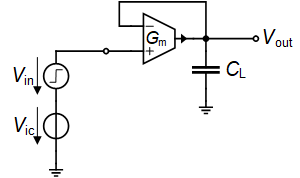
\includegraphics[keepaspectratio]{Figures/Voltage_follower.png}}

}

\caption{\label{fig-voltage_follower}Schematic of the OTA connected as a
voltage follower.}

\end{figure}%

In this section we will check the step response of the OTA operating as
a voltage follower as shown in Figure~\ref{fig-voltage_follower} with
its output connected to the negative input and with the same load
capacitance \(C_L =\) 1 \(pF\).

\subsection{Small-step}\label{small-step}

We start by imposing a small step \(\Delta V_{in} =\) 10 \(mV\) on top
of a common mode voltage \(V_{ic} =\) 0.6 \(V\). The simulation results
are shown in Figure~\ref{fig-ng_step_small} where
\(\Delta V_{in}(t) \triangleq V_{in+}(t) - V_{ic}\) and
\(\Delta V_{out}(t) \triangleq V_{out}(t) - V_{outq}\) with \(V_{outq}\)
the quiescent output voltage at the operating point before the step is
applied. \(\Delta V_{in}\) and \(\Delta V_{out}\) are compared to the
response of a single pole circuit having a cut-off frequency equal to
the \(GBW\). The difference between the simulation an the first-order
model is due to the larger estimated value of the \(GBW\) and the
additional poles introduced by the current mirrors.

\begin{figure}

\centering{

\pandocbounded{\includegraphics[keepaspectratio]{Symmetrical_OTA_files/figure-pdf/fig-ng_step_small-output-1.pdf}}

}

\caption{\label{fig-ng_step_small}Step response of the OTA as a voltage
follower for a small input step.}

\end{figure}%

\subsection{Large step}\label{large-step}

We now impose a larger step \(\Delta V_{in} =\) 300 \(mV\) on top of a
common mode voltage \(V_{ic} =\) 400 \(mV\). The simulation results are
shown in Figure~\ref{fig-ng_step_large} where
\(\Delta V_{in}(t) \triangleq V_{in+}(t) - V_{ic}\) and
\(\Delta V_{out}(t) \triangleq V_{out}(t) - V_{outq}\) with
\(V_{outq} \cong V_{ic}\) the quiescent output voltage at the operating
point before the step is applied. \(\Delta V_{in}\) and
\(\Delta V_{out}\) are compared to the response of a single pole circuit
having a cut-off frequency equal to the \(GBW\). We now observe the
effect of slew-rate which increases the settling time.

\begin{figure}

\centering{

\pandocbounded{\includegraphics[keepaspectratio]{Symmetrical_OTA_files/figure-pdf/fig-ng_step_large-output-1.pdf}}

}

\caption{\label{fig-ng_step_large}Step response of the OTA as a voltage
follower for a large input step highlighting the slew-rate effect.}

\end{figure}%

\section{Current and power
consumption}\label{current-and-power-consumption-1}

The total current consumption (without accounting for the current in
M\textsubscript{5a}) is given by \(I_{tot} =\) 1.120 \(\mu A\),
resulting in a total power consumption given by \(P =\) 1.344 \(\mu W\).
We can compare the current and power consumption of the Miller OTA to
the telescopic OTA \(I_{tot,telescopic} \cong\) 0.5 \(\mu A\). The
current and power consumption of the symmetrical cascode OTA is 2.240
times larger than that of the telescopic OTA for similar specifications
and performance.

\chapter{Conclusion}\label{conclusion}

This notebook presented the analysis, design and verification of the
symmetrical cascode OTA
\citeproc{ref-bib:krummenacher:el:1:4:1981}{{[}1{]}} for the IHP 130nm
SG13G2 open source PDK \citeproc{ref-bib:ihp:2025}{{[}5{]}}. The
detailed analysis provided all the equations that were then used in the
design phase to reach the target specifications. The design was then
performed using the inversion coefficient approach with the sEKV
transistor model \citeproc{ref-bib:enz:book:2006}{{[}2{]}}
\citeproc{ref-bib:enz:sscmag:autumn:2017}{{[}3{]}}
\citeproc{ref-bib:enz:sscmag:winter:2017}{{[}4{]}}. The theoretical
performance resulting from the design were then evaluated.

The design was then verified by simulation using ngspice with the PSP
compact model \citeproc{ref-bib:psp103.6:2017}{{[}7{]}} and the
parameters provided by the IHP 130nm SG13G2 open source PDK
\citeproc{ref-bib:ihp:2025}{{[}5{]}}. Because of the high output
resistance and the structural mismatch in the current mirrors due to the
output conductances, the open-loop quiescent output voltage was too low,
pushing some transistors out of saturation. The OTA was then simulated
in closed-loop as a voltage follower in order to extract the offset
voltage required to bring the quiescent output voltage in open-loop back
to the high gain region. After carefully checking the operating point,
the large-signal transfer characteristic was simulated. Then the
small-signal transfer function of the OTA connected as a voltage
follower was simulated. The open-loop transfer function was then
simulated making sure the OTA was biased in the high gain region. The
transfer function was then compared to the that extracted from the
closed-loop simulation showing a reasonable correspondance below the
unity gain frequency. The simulations have shown that the gain-bandwidth
product \(GBW\) is right on target. The DC gain is also achieved despite
the high output conductances of nMOS transistors.

The input-referred noise was then simulated and compared to the
theoretical estimation which is reasonably close. The contributions of
the various transistors to the input-referred white noise were then
extracted from the noise simulation and compared to the theoretical
estimation. It was shown that the total white noise was slightly above
the theoretical estimation. This is probably due to the high noise
excess factor of pMOS transistors which are almost two times larger than
the value obtained from the sEKV model. It was shown that the flicker
noise of the current mirrors is about equal to that of the differential
pair. Finally, the simulations have confirmed that the noise
contributions of the cascode transistors are perfectly negligible.

The input common-mode voltage range was then simulated with the OTA
connected as a voltage follower.The input voltage is limited to
\(0.9\,V\).

Finally, the small-signal step response was simulated and succesfully
compared to the response of single-pole system. The step-response with a
large input step highlighted the effect of slew-rate.

This design has highlighted an important drawback of this technology,
namely the high output conductance of nMOS transistors and even for
long-channel.

Despite the compact model that was used for the simulation is not the
EKV compact model but the PSP model, the simulation results are
reasonably close to the theoretical estimations made with the sEKV
model. Of course this required to extract the sEKV parameters for the
IPHP SG13G2 technology.

\chapter*{References}\label{references}
\addcontentsline{toc}{chapter}{References}

\phantomsection\label{refs}
\begin{CSLReferences}{0}{0}
\bibitem[\citeproctext]{ref-bib:krummenacher:el:1:4:1981}
\CSLLeftMargin{{[}1{]} }%
\CSLRightInline{F. Krummenacher, {``{High voltage gain CMOS OTA for
micropower SC filters},''} \emph{Electronics Letters}, vol. 17, no. 4,
pp. 160--162, 1981.}

\bibitem[\citeproctext]{ref-bib:enz:book:2006}
\CSLLeftMargin{{[}2{]} }%
\CSLRightInline{C. C. Enz and E. A. Vittoz, \emph{{Charge-Based MOS
Transistor Modeling - The EKV Model for Low-Power and RF IC Design}},
1st ed. John Wiley, 2006.}

\bibitem[\citeproctext]{ref-bib:enz:sscmag:autumn:2017}
\CSLLeftMargin{{[}3{]} }%
\CSLRightInline{C. Enz, F. Chicco, and A. Pezzotta, {``{Nanoscale MOSFET
Modeling: Part 1: The Simplified EKV Model for the Design of Low-Power
Analog Circuits},''} \emph{IEEE Solid-State Circuits Magazine}, vol. 9,
no. 3, pp. 26--35, 2017.}

\bibitem[\citeproctext]{ref-bib:enz:sscmag:winter:2017}
\CSLLeftMargin{{[}4{]} }%
\CSLRightInline{C. Enz, F. Chicco, and A. Pezzotta, {``{Nanoscale MOSFET
Modeling: Part 2: Using the Inversion Coefficient as the Primary Design
Parameter},''} \emph{IEEE Solid-State Circuits Magazine}, vol. 9, no. 4,
pp. 73--81, 2017.}

\bibitem[\citeproctext]{ref-bib:ihp:2025}
\CSLLeftMargin{{[}5{]} }%
\CSLRightInline{IHP, {``{IHP SG13G2 Open Source PDK}.''}
\url{https://github.com/IHP-GmbH/IHP-Open-PDK}, 2025.}

\bibitem[\citeproctext]{ref-bib:ngspice:2024}
\CSLLeftMargin{{[}6{]} }%
\CSLRightInline{Holger Vogt, Giles Atkinson, Paolo Nenzi, {``{Ngspice
User's Manual Version 43}.''}
\url{https://ngspice.sourceforge.io/docs/ngspice-43-manual.pdf}, 2024.}

\bibitem[\citeproctext]{ref-bib:psp103.6:2017}
\CSLLeftMargin{{[}7{]} }%
\CSLRightInline{G.D.J. Smit, A.J. Scholten, D.B.M. Klaassen, O. Rozeau,
S. Martinie, T. Poiroux and J.C. Barbé, {``{PSP 103.6 - The PSP model is
a joint development of CEA-Leti and NXP Semiconductors}.''}
\url{https://www.cea.fr/cea-tech/leti/pspsupport/Documents/psp103p6_summary.pdf},
2017.}

\bibitem[\citeproctext]{ref-bib:krummenacher:el:17:13:1981}
\CSLLeftMargin{{[}8{]} }%
\CSLRightInline{F. Krummenacher, E. Vittoz, and M. Degrauwe, {``{Class
AB CMOS amplifier micropower SC filters},''} \emph{Electronics Letters},
vol. 17, no. 13, pp. 433--435, 1981.}

\bibitem[\citeproctext]{ref-bib:degrauwe:jssc:17:3:june:1982}
\CSLLeftMargin{{[}9{]} }%
\CSLRightInline{M. G. Degrauwe, J. Rijmenants, E. A. Vittoz, and H. J.
D. Man, {``{Adaptive biasing CMOS amplifiers},''} \emph{IEEE Journal of
Solid-State Circuits}, vol. 17, no. 3, pp. 522--528, 1982.}

\bibitem[\citeproctext]{ref-bib:openvaf:2025}
\CSLLeftMargin{{[}10{]} }%
\CSLRightInline{SemiMod GmbH, {``{Open VAF}.''}
\url{https://openvaf.semimod.de/docs/getting-started/introduction/},
2025.}

\bibitem[\citeproctext]{ref-bib:dwarning:2024}
\CSLLeftMargin{{[}11{]} }%
\CSLRightInline{Dietmar Warning, {``{Verilog-A Models for Circuit
Simulation}.''} \url{https://github.com/dwarning/VA-Models}, 2024.}

\bibitem[\citeproctext]{ref-bib:iccap:2008}
\CSLLeftMargin{{[}12{]} }%
\CSLRightInline{Agilent Technologies, {``{IC-CAP 2008, Nonlinear Device
Models - Volume 1}.''}
\url{https://people.ece.ubc.ca/robertor/Links_files/Files/ICCAP-2008-doc/pdf/icmdl.pdf},
2008.}

\end{CSLReferences}




\end{document}
